\documentclass[conference]{IEEEtran}
\IEEEoverridecommandlockouts

\usepackage{fontspec}
\usepackage{polyglossia}
\setmainlanguage{portuges}
\usepackage{cite}
\usepackage{amsmath,amssymb,amsfonts}
\usepackage{graphicx}
\usepackage{textcomp}
\usepackage{xcolor}
\usepackage{booktabs}
\usepackage{array}
\usepackage{multirow}
\usepackage{url}
\usepackage[hidelinks]{hyperref}

\def\BibTeX{{\rm B\kern-.05em{\sc i\kern-.025em b}\kern-.08em
    T\kern-.1667em\lower.7ex\hbox{E}\kern-.125emX}}

\begin{document}

\title{Mineração de Dados, Tradução Semântica Híbrida via IA, Visualização Multidimensional e Aprendizado de Máquina no Turfe Japonês de Elite (2002--2025)\\
{\footnotesize \textnormal{Disciplina de Ciência dos Dados --- Centro Federal de Educação Tecnológica de Minas Gerais (CEFET-MG)}}
}

\author{\IEEEauthorblockN{Arthur De Oliveira Mendonça}
\IEEEauthorblockA{\textit{Departamento de Computação e Mecatrônica} \\
\textit{Centro Federal de Educação Tecnológica de Minas Gerais (CEFET-MG --- Campus Divinópolis)}\\
Divinópolis, Minas Gerais, Brasil \\
Repositório Oficial: \url{https://github.com/ImArthz/AEDS2_jra_analysis} --- DOI: \url{https://doi.org/10.5281/zenodo.23681764}}
}

\maketitle

\begin{abstract}
Este artigo apresenta um ecossistema completo de Engenharia e Ciência dos Dados voltado à extração, higienização estrutural, tradução semântica assistida por Inteligência Artificial, visualização multidimensional e modelagem preditiva de 24 anos de histórico oficial (2002--2025) das corridas de elite (\textit{Graded Races}: G1, G2 e G3) da \textit{Japan Racing Association} (JRA), integradas às árvores genealógicas ascendentes de 5 gerações do \textit{Japan Bloodhorse Information System} (JBIS). A base consolidada compreende 3.216 corridas, 33.409 participações validadas, 8.209 cavalos Puro-Sangue Inglês e 504.074 nós genealógicos mapeados sem quebras de integridade referencial. Para superar barreiras linguísticas severas (leituras antroponímicas \textit{Nanori}, prefixos tradicionais \textit{Kanmei} e taxonomia biológica) e anomalias históricas de layout HTML (fusão de colunas entre 2006 e 2018 e inversão topológica DFS/BFS), desenvolveu-se um motor híbrido de tradução em três camadas acoplado à API Google Gemini (\textit{cache} de 29.159 termos) e algoritmos determinísticos de realinhamento vetorial. A análise inferencial comprovou especialização genética extrema por superfície ($\chi^2 = 739,99, p = 2,43 \times 10^{-107}, V = 0,2514$) e regime de distância ($\chi^2 = 2237,47, p = 3,71 \times 10^{-317}, V = 0,2523$; ANOVA $F = 16,46, p = 1,68 \times 10^{-35}$). A aplicação do algoritmo PageRank ($d = 0,85$) sobre a rede de confrontos ($r = 0,8799$ com pódios) permitiu identificar ``Diamantes Injustiçados'' com zero vitórias Graded, mas altíssimo prestígio competitivo (\textit{Sounds of Earth}, \#32 entre 8.135 cavalos). A clusterização não-supervisionada K-Means++ projetada via PCA 2D (63,4\%
de variância explicada) segmentou 106 garanhões em quatro arquétipos zootécnicos, enquanto o classificador supervisionado \textit{Random Forest} avaliado em divisão temporal estrita (\textit{Out-of-Time}: 2016--2018, $N = 5.889$, \textit{Zero Data Leakage}) atingiu $\text{ROC-AUC} = 0,7260$ (IC 95\%
$[0,7109;\; 0,7389]$), revelando que o histórico prévio do jóquei (29,8\%
de importância de Gini) e do cavalo (22,7\%)
lideram o poder preditivo de pódio. Por fim, disponibilizam-se suítes interativas em \textit{Apache Superset / ECharts} (13 gráficos) e uma arena gamificada de 520 cards colecionáveis (TCG).
\end{abstract}

\begin{IEEEkeywords}
Ciência dos Dados, Turfe Japonês (JRA/JBIS), Tradução Semântica por LLM, PageRank Esportivo, Especialização Genética, K-Means++ PCA, Random Forest, Visualização Multidimensional, Apache Superset.
\end{IEEEkeywords}

\section{Introdução}
O turfe japonês organizado pela \textit{Japan Racing Association} (JRA) constitui a indústria hípica e de melhoramento genético de Puro-Sangue Inglês (\textit{Thoroughbred}) mais tecnologicamente avançada e financeiramente expressiva do mundo, movimentando bilhões de dólares anualmente e mantendo registros genealógicos rigorosos através do \textit{Japan Bloodhorse Information System} (JBIS) [1, 2]. Ao longo das últimas duas décadas e meia (2002--2025), a introdução de linhagens fundadoras norte-americanas e europeias --- notadamente \textit{Sunday Silence (USA)}, \textit{Brian's Time (USA)} e descendentes de \textit{Northern Dancer (CAN)} --- remodelou profundamente a arquitetura genética dos competidores japoneses, culminando em campeões mundiais como \textit{Deep Impact}, \textit{Orfevre}, \textit{Almond Eye} e \textit{Kitasan Black}.

Sob a ótica da Ciência dos Dados, esse domínio oferece um laboratório empírico excepcionalmente rico: cada corrida de elite (\textit{Graded Race} de Grau 1, Grau 2 ou Grau 3) registra variáveis físicas, cinemáticas, ambientais, humanas e biológicas de alta precisão. Contudo, a exploração científica desses dados por pesquisadores ocidentais esbarra historicamente na ausência de bases públicas relacionais higienizadas e padronizadas em língua inglesa, bem como na complexidade de integrar resultados esportivos tabulares com árvores genealógicas multigeracionais.

Este trabalho documenta o ciclo completo de Ciência dos Dados aplicado a 24 temporadas da JRA (2002--2025) e 5 gerações de ancestrais do JBIS, abrangendo desde a coleta automatizada (\textit{Web Scraping}) e o tratamento de anomalias estruturais até a inferência estatística, modelagem preditiva supervisionada e não-supervisionada, visualização multidimensional baseada na taxonomia do \textit{DataViz Project} e do \textit{Apache Superset 6.1} [8, 9] e gamificação científica via \textit{Procedural Game Design}.

\section{Descrição do Problema}
A construção de uma matriz analítica confiável a partir dos portais legados da JRA e do JBIS exigiu a resolução de quatro problemas estruturais críticos:
\begin{enumerate}
    \item \textbf{Fragmentação e Mutação Histórica de Layouts HTML (2002--2025):} Os registros da JRA atravessam três gerações tecnológicas da web (tabelas HTML4 estáticas codificadas em \texttt{Shift\_JIS} nos anos 2000 até estruturas HTML5 em \texttt{UTF-8}). Auditorias nos dados brutos revelaram que, entre 2006 e 2018, as tabelas da JRA fundiram as colunas de Sexo e Idade em uma única célula (coluna \textit{Seirei} [\texttt{Sexo+Idade}], ex.: \texttt{Male-4}), deslocando em uma posição todos os índices subsequentes do \textit{parser} (Jóquei, Tempo Final, Margem, Treinador e Peso Corporal) em 25.014 registros, além de omitirem a classificação explícita de \textit{grade} em 1.834 provas de 2002--2015 e abreviarem superfícies de areia (\textit{Da} / \textit{Dirt}) e obstáculos (\textit{Sho} / \textit{Obstacle}).
    \item \textbf{Inversão Topológica DFS vs. BFS na Árvore de 5 Gerações:} O portal JBIS renderiza os 62 ancestrais de cada animal ($2^1 + 2^2 + 2^3 + 2^4 + 2^5 = 62$) em uma tabela HTML com \texttt{rowspan} progressivo ordenada em Busca em Largura (\textit{Breadth-First Search --- BFS}, geração por geração), enquanto rotuladores sequenciais ingênuos indexam os caminhos (\texttt{S}, \texttt{SS}, \texttt{SSS}...) em Busca em Profundidade (\textit{Depth-First Search --- DFS}), corrompendo as conexões pai-filho em 504.074 nós.
    \item \textbf{Intraduzibilidade Fonética e Ambiguidade Semântica do Japonês:} Nomes de cavalos em \textit{Katakana} representam conceitos em inglês, francês ou italiano (\textit{Di-pu In-pa-ku-to} $\to$ \textit{Deep Impact}; \textit{O-ru-fe-vu-ru} $\to$ \textit{Orfevre}), enquanto nomes de jóqueis e treinadores em \textit{Kanji} utilizam leituras antroponímicas especiais (\textit{Nanori}, como \textit{Take Yutaka} $\to$ \textit{Yutaka Take}), criadores utilizam abreviaturas societárias (\textit{Yugen Gaisha} $\to$ \textit{Co., Ltd.}) e pelagens exigem taxonomia zootécnica (\textit{Kage} $\to$ \textit{Bay}). Conversores fonéticos convencionais geram ruído severo (\texttt{"Diipu Inpakuto"}, \texttt{"Taketoyo"}, \texttt{"(Ari)"}, \texttt{"Kage"}), inviabilizando análises internacionais.
    \item \textbf{Cegueira da Contagem Simples de Vitórias e Vazamento Temporal (\textit{Data Leakage}):} Avaliar cavalos apenas pelo número bruto de vitórias subestima competidores que enfrentaram a elite absoluta em provas de Grau 1 (terminando repetidamente em 2º ou 3º lugar contra lendas históricas) e superestima vencedores de provas regionais de Grau 3. Adicionalmente, modelos de Machine Learning que utilizam estatísticas agregadas de fim de carreira sofrem de vazamento temporal (\textit{look-ahead bias}).
\end{enumerate}

\section{Objetivos do Trabalho}
\subsection{Objetivo Geral}
Projetar, validar e disponibilizar publicamente uma base de dados relacional e de grafos bilíngue (Japonês/Inglês) sobre 24 anos de corridas de elite da JRA e genealogia de 5 gerações do JBIS, aplicando técnicas rigorosas de inferência estatística, aprendizado de máquina sem vazamento temporal e visualização multidimensional para responder como a herança genética e o fator humano determinam a aptidão física e o sucesso competitivo no turfe.

\subsection{Objetivos Específicos}
\begin{itemize}
    \item Extrair e higienizar 100\%
das corridas G1, G2 e G3 da JRA (2002--2025) e árvores de 5 gerações do JBIS na Terceira Forma Normal (3NF), corrigindo o deslocamento vetorial de 25.014 linhas e a bijeção DFS$\to$BFS em 504.074 ancestrais com zero erros de validação (QA);
    \item Construir um motor híbrido de tradução semântica assistido por Grandes Modelos de Linguagem (Google Gemini API) para traduzir 29.159 termos técnicos e nomes próprios para o inglês oficial;
    \item Testar estatisticamente a hipótese de especialização genética ($H_1$) por superfície e distância ($\chi^2$, $V$ de Cramér, ANOVA One-Way e Kruskal-Wallis) e calcular o Coeficiente de Endogamia de Wright ($F_X$);
    \item Modelar o prestígio competitivo via algoritmo PageRank ($H_2$) para identificar anomalias de alto desempenho sem vitórias Graded (``Diamantes Injustiçados'');
    \item Segmentar garanhões reprodutores via clusterização não-supervisionada K-Means++ e redução de dimensionalidade PCA 2D, e treinar classificadores supervisionados (\textit{Random Forest} e Regressão Logística L2) em divisão cronológica estrita para predição de pódio (\mbox{Top-3});
    \item Desenvolver visualizações multidimensionais de alta resolução (300 DPI), uma suíte interativa baseada no motor do \textit{Apache Superset 6.1} (\textit{Apache ECharts}) e uma arena gamificada de cards (TCG).
\end{itemize}

\section{Metodologia}
O pipeline metodológico foi estruturado em seis módulos integrados em linguagem Python, detalhados a seguir.

\subsection{Técnicas de Extração de Dados (\textit{Web Scraping})}
A coleta primária foi dividida em dois extratores HTTP orientados a eventos (\texttt{src/scraper\_jra.py} e \texttt{src/scraper\_pedigree.py}). No portal da JRA, o extrator percorre os calendários anuais de provas Graded (\textit{Jusho}) de 2002 a 2025 utilizando \texttt{requests} e \texttt{BeautifulSoup4} (\textit{parser} C \texttt{lxml}), aplicando decodificação adaptativa (\texttt{Shift\_JIS}/\texttt{CP932} para páginas legadas e \texttt{UTF-8} para páginas modernas). No portal JBIS, para cada um dos 8.209 cavalos únicos identificados nas pistas, o extrator consulta o perfil biológico (listas semânticas \texttt{<dt>/<dd>} contendo ganhos em \textit{Man-Yen} convertidos por $\times 10.000$, pelagem, criador e proprietário) e a tabela genealógica de 5 gerações (\texttt{/horse/ped/}). Para garantir resiliência e respeito aos servidores de origem, implementou-se \textit{Skip Logic} em $O(1)$ via consulta prévia ao banco SQLite (modo WAL --- \textit{Write-Ahead Logging}), \textit{throttling} configurável ($1,5\text{s}$ a $2,0\text{s}$) e \textit{Exponential Backoff} ($2^k\text{s}$) contra falhas de rede.

\subsection{Tratamento de Dados, Natureza das Variáveis e Codificação de Variáveis Categóricas}
A base consolidada foi modelada em cinco tabelas relacionais na Terceira Forma Normal (3NF): \texttt{races} (3.216 corridas), \texttt{race\_entries} (33.409 participações), \texttt{horses} (8.209 cavalos), \texttt{pedigree} (8.202 relações diretas pai/mãe/avô materno) e \texttt{pedigree\_tree} (504.074 nós ancestrais de 5 gerações). A Tabela~I sintetiza a taxonomia estatística das variáveis, seus tipos primitivos e o tratamento aplicado.

\begin{table}[htbp]
\caption{Natureza Estatística dos Dados, Tipos e Tratamento Aplicado}
\begin{center}
\renewcommand{\arraystretch}{1.15}
\resizebox{\columnwidth}{!}{%
\begin{tabular}{p{2.1cm}p{1.9cm}p{3.9cm}}
\toprule
\textbf{Variável} & \textbf{Natureza / Tipo} & \textbf{Tratamento e Codificação} \\
\midrule
\texttt{distance} (m) & Quant. Contínua (\texttt{float}) & Imputação via NFKC + categorização ordinal em 4 regimes. \\
\texttt{horse\_mass\_kg} & Quant. Contínua (\texttt{float}) & Extração via Regex \texttt{\^{}(\textbackslash d\{3\})} de \texttt{"486Kg(+2)"} e mediana no treino. \\
\texttt{weight} (kg) & Quant. Contínua (\texttt{float}) & Remoção de sufixo \texttt{"kg"} (\texttt{56.0kg} $\to 56,0$) e padronização Z-score. \\
\texttt{total\_earnings} & Quant. Contínua (\texttt{float}) & Conversão de \textit{Man-Yen} ($\times 10^4$) para Ienes (¥) e escala em milhões. \\
\texttt{inbreeding\_fx} & Quant. Contínua (\texttt{float}) & Cálculo exato de Wright: $F_X = \sum (1/2)^{n_S + n_D - 1}$ em 5 gerações. \\
\texttt{year}, \texttt{age}, \texttt{position} & Quant. Discreta (\texttt{int}) & Decomposição de \textit{Seirei} (\texttt{Sexo+Idade} $\to 4$), filtro $\text{pos} < 90$ e alvo binário $\le 3$. \\
\texttt{grade} (G1/G2/G3) & Qualit. Ordinal (\texttt{str}) & Codificação ordinal ponderada: $\text{G1}=1,0;\; \text{G2}=0,7;\; \text{G3}=0,5$. \\
\texttt{surface}, \texttt{sex}, \texttt{color} & Qualit. Nominal (\texttt{str}) & Tradução determinística $O(1)$ e \textit{One-Hot / Dummy} (\texttt{is\_turf}, \texttt{is\_female}). \\
\texttt{jockey}, \texttt{trainer}, \texttt{sire}, \texttt{dam\_sire} & Qualit. Nominal Alta Cardin. & Tradução Híbrida Gemini IA + \textit{Bayesian Shifted Expanding-Window Target Encoding}. \\
\bottomrule
\end{tabular}%
}
\label{tab:natureza_dados}
\end{center}
\end{table}

\subsubsection{Tratamento Especial de Variáveis Categóricas}
As variáveis categóricas receberam três níveis de engenharia de atributos:
\begin{itemize}
    \item \textbf{Normalização Unicode NFKC e Tradução Híbrida em 3 Camadas (\texttt{src/hybrid\_translator.py}):} Caracteres de largura total (\textit{Full-Width}) foram normalizados via \texttt{unicodedata.normalize('NFKC')}. Na Camada 1, dicionários determinísticos $O(1)$ traduziram categorias fechadas: superfícies (\textit{Turf}, \textit{Dirt}, \textit{Obstacle}), hipódromos (os 10 circuitos da JRA), sexo (\textit{Male}, \textit{Female}, \textit{Gelding}) e a taxonomia biológica de pelagens (\textit{Bay}, \textit{Dark Bay}, \textit{Chestnut}, \textit{Dark Chestnut}, \textit{Grey}, \textit{Brown}, \textit{Black}, \textit{White}). Na Camada 2, desacoplaram-se sufixos geográficos \texttt{(USA)/(GB)} via Regex, reduzindo 39.533 strings brutas para 23.511 radicais japoneses únicos, traduzidos por um pool multi-modelo da API Google Gemini (\texttt{gemini-3.5-flash-lite}, \texttt{gemini-3.5-flash}, \texttt{gemini-3.7-flash}) com saída estrita em JSON (\texttt{temperature=0.0}). Na Camada 3, regras de prefixos tradicionais (\textit{Kanmei}: \textit{Symboli}, \textit{Mejiro}, \textit{Daiwa}, \textit{Meisho}) consolidaram um dicionário validado de \textbf{29.159 termos} (\path{data/gemini_cache.json}) com zero caracteres japoneses residuais.
    \item \textbf{Codificação de Variáveis Categóricas para Machine Learning sem Vazamento Temporal:} Para variáveis nominais de baixa cardinalidade (\texttt{surface}, \texttt{sex}), aplicou-se codificação binária (\texttt{is\_turf}, \texttt{is\_female}); para \texttt{grade}, aplicou-se codificação ordinal (\texttt{grade\_weight} $\in \{1,0; 0,7; 0,5\}$). Para variáveis categóricas de alta cardinalidade (\texttt{horse\_name} com 8.209 categorias, \texttt{jockey} com 398, \texttt{trainer} com 412 e \texttt{sire} com 985), o \textit{One-Hot Encoding} geraria uma matriz esparsa de mais de 10.000 colunas com severo sobreajuste (\textit{overfitting}). Implementou-se, portanto, o \textbf{\textit{Shifted Expanding-Window Bayesian Target Encoding}}: para cada entidade $e$ na corrida cronológica $t$, a taxa histórica prévia de pódio é calculada exclusivamente sobre as corridas estritamente anteriores ($1 \dots t-1$) com suavização bayesiana (\textit{m-estimate}):
    \begin{equation}
        \hat{R}_{e}^{(t)} = \frac{\sum_{i=1}^{t-1} \mathbb{I}(e_i = e \land y_i = 1) + m \cdot \bar{y}_{\text{global}}}{\sum_{i=1}^{t-1} \mathbb{I}(e_i = e) + m}
    \end{equation}
    onde $\bar{y}_{\text{global}} = 0,20$ é a probabilidade a priori de pódio e $m \in \{3, 15, 20\}$ é o peso de suavização empírica. Analogamente, criaram-se termos de interação genética prévia (\texttt{sire\_surface\_affinity} e \texttt{sire\_distance\_affinity}) cruzando o garanhão com a superfície e a categoria de distância da prova.
\end{itemize}

\subsubsection{Sanitização Estrutural e Bijeção Genealógica (\texttt{src/clean\_data.py})}
O algoritmo de limpeza realinhou in-place as 25.014 linhas deslocadas de 2004--2018 (desmembrando o par Sexo+Idade e restaurando 100\%
da cobertura de Jóquei, Treinador, Idade e Peso em todas as 33.409 participações), expurgou em cascata 15 registros espúrios oriundos de tabelas de rateio de apostas de 2004 e imputou 100\%
de \texttt{grade}, \texttt{surface} e \texttt{distance} nas 3.216 corridas via auto-junção histórica. Na tabela \texttt{pedigree\_tree} (504.074 linhas), aplicou-se a bijeção matemática exata $1\text{-para-}1$ que converte os 62 rótulos de caminho da ordem DFS para a ordem BFS real do HTML do JBIS, além de desambiguar 15 campeões de G1 homônimos (\textit{Almond Eye}, \textit{Kitasan Black}, \textit{Vodka}, \textit{Maurice}, etc.). A auditoria final (\texttt{src/validate\_data.py}) atestou \textbf{0 erros e 0 avisos}.

\subsection{Justificativa de Adaptação de Bibliotecas e Ferramentas}
Em conformidade com as diretrizes metodológicas da disciplina, registram-se duas adaptações justificadas em relação à proposta inicial:
\begin{enumerate}
    \item \textbf{Migração de Transliteradores Fonéticos (\texttt{pykakasi}) para Arquitetura Híbrida com LLM (Google Gemini API):} Testes preliminares demonstraram que bibliotecas puramente fonéticas corrompiam a semântica de nomes ocidentais grafados em Katakana e nomes humanos em Kanji, exigindo a criação do motor híbrido em 3 camadas (\texttt{src/hybrid\_translator.py}).
    \item \textbf{Implementação Vetorizada em \texttt{NumPy}/\texttt{Pandas} e Adoção do Motor \textit{Apache ECharts 5.5} (\textit{Apache Superset 6.1}) e \textit{Gephi}:} No ambiente de execução Python 3.15 (\texttt{cp315}), pacotes legados dependentes de compilação Fortran/C (\texttt{scipy}) não possuíam rodas binárias pré-compiladas para Windows. Para assegurar execução instantânea e autossuficiente, implementamos todos os testes estatísticos ($\chi^2$, ANOVA $F$, Kruskal-Wallis $H$, aproximação normal de Wilson-Hilferty), o algoritmo \textit{Power Iteration} do PageRank, o \textit{K-Means++} com decomposição SVD para PCA 2D, a Regressão Logística L2 e o ensemble \textit{Random Forest} (árvores CART com importância de Gini e Bootstrap IC 95\%)
diretamente em álgebra linear vetorizada via \texttt{NumPy} e \texttt{Pandas}. Para a visualização de dados, além de \texttt{Matplotlib} e \texttt{Seaborn}, incorporaram-se o \textbf{Gephi} (para renderização vetorial ForceAtlas2 de grafos) e o motor \textbf{Apache ECharts 5.5} (núcleo gráfico oficial do \textbf{Apache Superset 6.1}) para a construção dos dashboards interativos web.
\end{enumerate}

\subsection{Modelagem em Grafos, Inferência Estatística e Machine Learning}
\begin{itemize}
    \item \textbf{PageRank Esportivo e Endogamia de Wright ($F_X$):} Na rede direcionada de competição $G_c = (V_c, E_c, W)$, cada corrida gera arestas direcionadas dos perdedores para os ocupantes do pódio ponderadas por $w(\text{G1})=1,0$, $w(\text{G2})=0,7$ e $w(\text{G3})=0,5$. O vetor de prestígio PageRank ($d = 0,85$) foi resolvido até convergência $\|\pi^{(k)} - \pi^{(k-1)}\|_1 < 10^{-9}$. No DAG genealógico $G_p$ de 5 gerações, o Coeficiente de Endogamia de Wright foi calculado exatamente sobre todos os Menores Ancestrais Comuns (LCA) paternos e maternos: $F_X = \sum_{A \in \text{LCA}} (1/2)^{n_S + n_D - 1}$.
    \item \textbf{Clusterização K-Means++ \& PCA 2D:} Os 106 principais garanhões ($\ge 50$ largadas da prole) foram padronizados (Z-score) sobre 6 atributos zootécnicos (\% Grama, Distância Média, Taxa de Vitória, Taxa de Pódio, \% Vitórias G1 e PageRank Médio dos Filhos), avaliados por \textit{Silhouette Score} para $k \in \{2 \dots 7\}$ e projetados nos dois primeiros componentes principais via Decomposição em Valores Singulares ($\mathbf{X} = \mathbf{U}\mathbf{\Sigma}\mathbf{V}^T$).
    \item \textbf{Classificação Supervisionada (\textit{Out-of-Time}):} Para prever a chegada no pódio ($\text{target\_top3} = \mathbb{I}(\text{position} \le 3)$), o dataset foi particionado cronologicamente em \textbf{Treino (2002--2013)}, \textbf{Validação (2014--2015)} e \textbf{Teste Out-of-Time (2016--2018, $N = 5.889$)}, utilizando 17 variáveis estritamente anteriores à largada. Avaliaram-se três modelos: Baseline Estratificado, Regressão Logística L2 balanceada e \textit{Random Forest Classifier} (45 árvores CART com \textit{bagging} e amostragem $\sqrt{p}$ de atributos por nó).
\end{itemize}

\section{Visualização de Dados e Análise dos Resultados}
Seguindo os princípios de percepção visual do \textit{DataViz Project} e do \textit{Apache Superset 6.1} [8, 9], geraram-se representações estáticas em 300 DPI (\path{src/generate_plots.py}, \path{src/ml_analysis.py} e \path{src/generate_advanced_viz.py}) e duas aplicações web interativas analisadas a seguir.

\subsection{Dominância Paterna, Premiação Vitalícia e Fluxo Aluvial (Sankey)}
A Fig.~1 apresenta a distribuição dos 10 maiores garanhões por número de filhos únicos em corridas Graded e os 10 maiores ganhadores financeiros da história da JRA. Verifica-se a hegemonia absoluta de \textbf{Deep Impact} (289 filhos únicos em provas Graded, 1.541 largadas e 46 títulos de G1) e de seu pai \textbf{Sunday Silence (USA)} (281 filhos, 1.793 largadas e 42 títulos de G1), seguidos por \textbf{King Kamehameha} (212 filhos), \textbf{Fuji Kiseki} (173) e \textbf{Stay Gold} (133). No ranking financeiro, \textbf{Almond Eye} (¥19,15 Bilhões / 1.915,3 milhões de ienes) e \textbf{Kitasan Black} (¥18,77 Bilhões) lideram a era moderna.

\begin{figure}[htbp]
\centerline{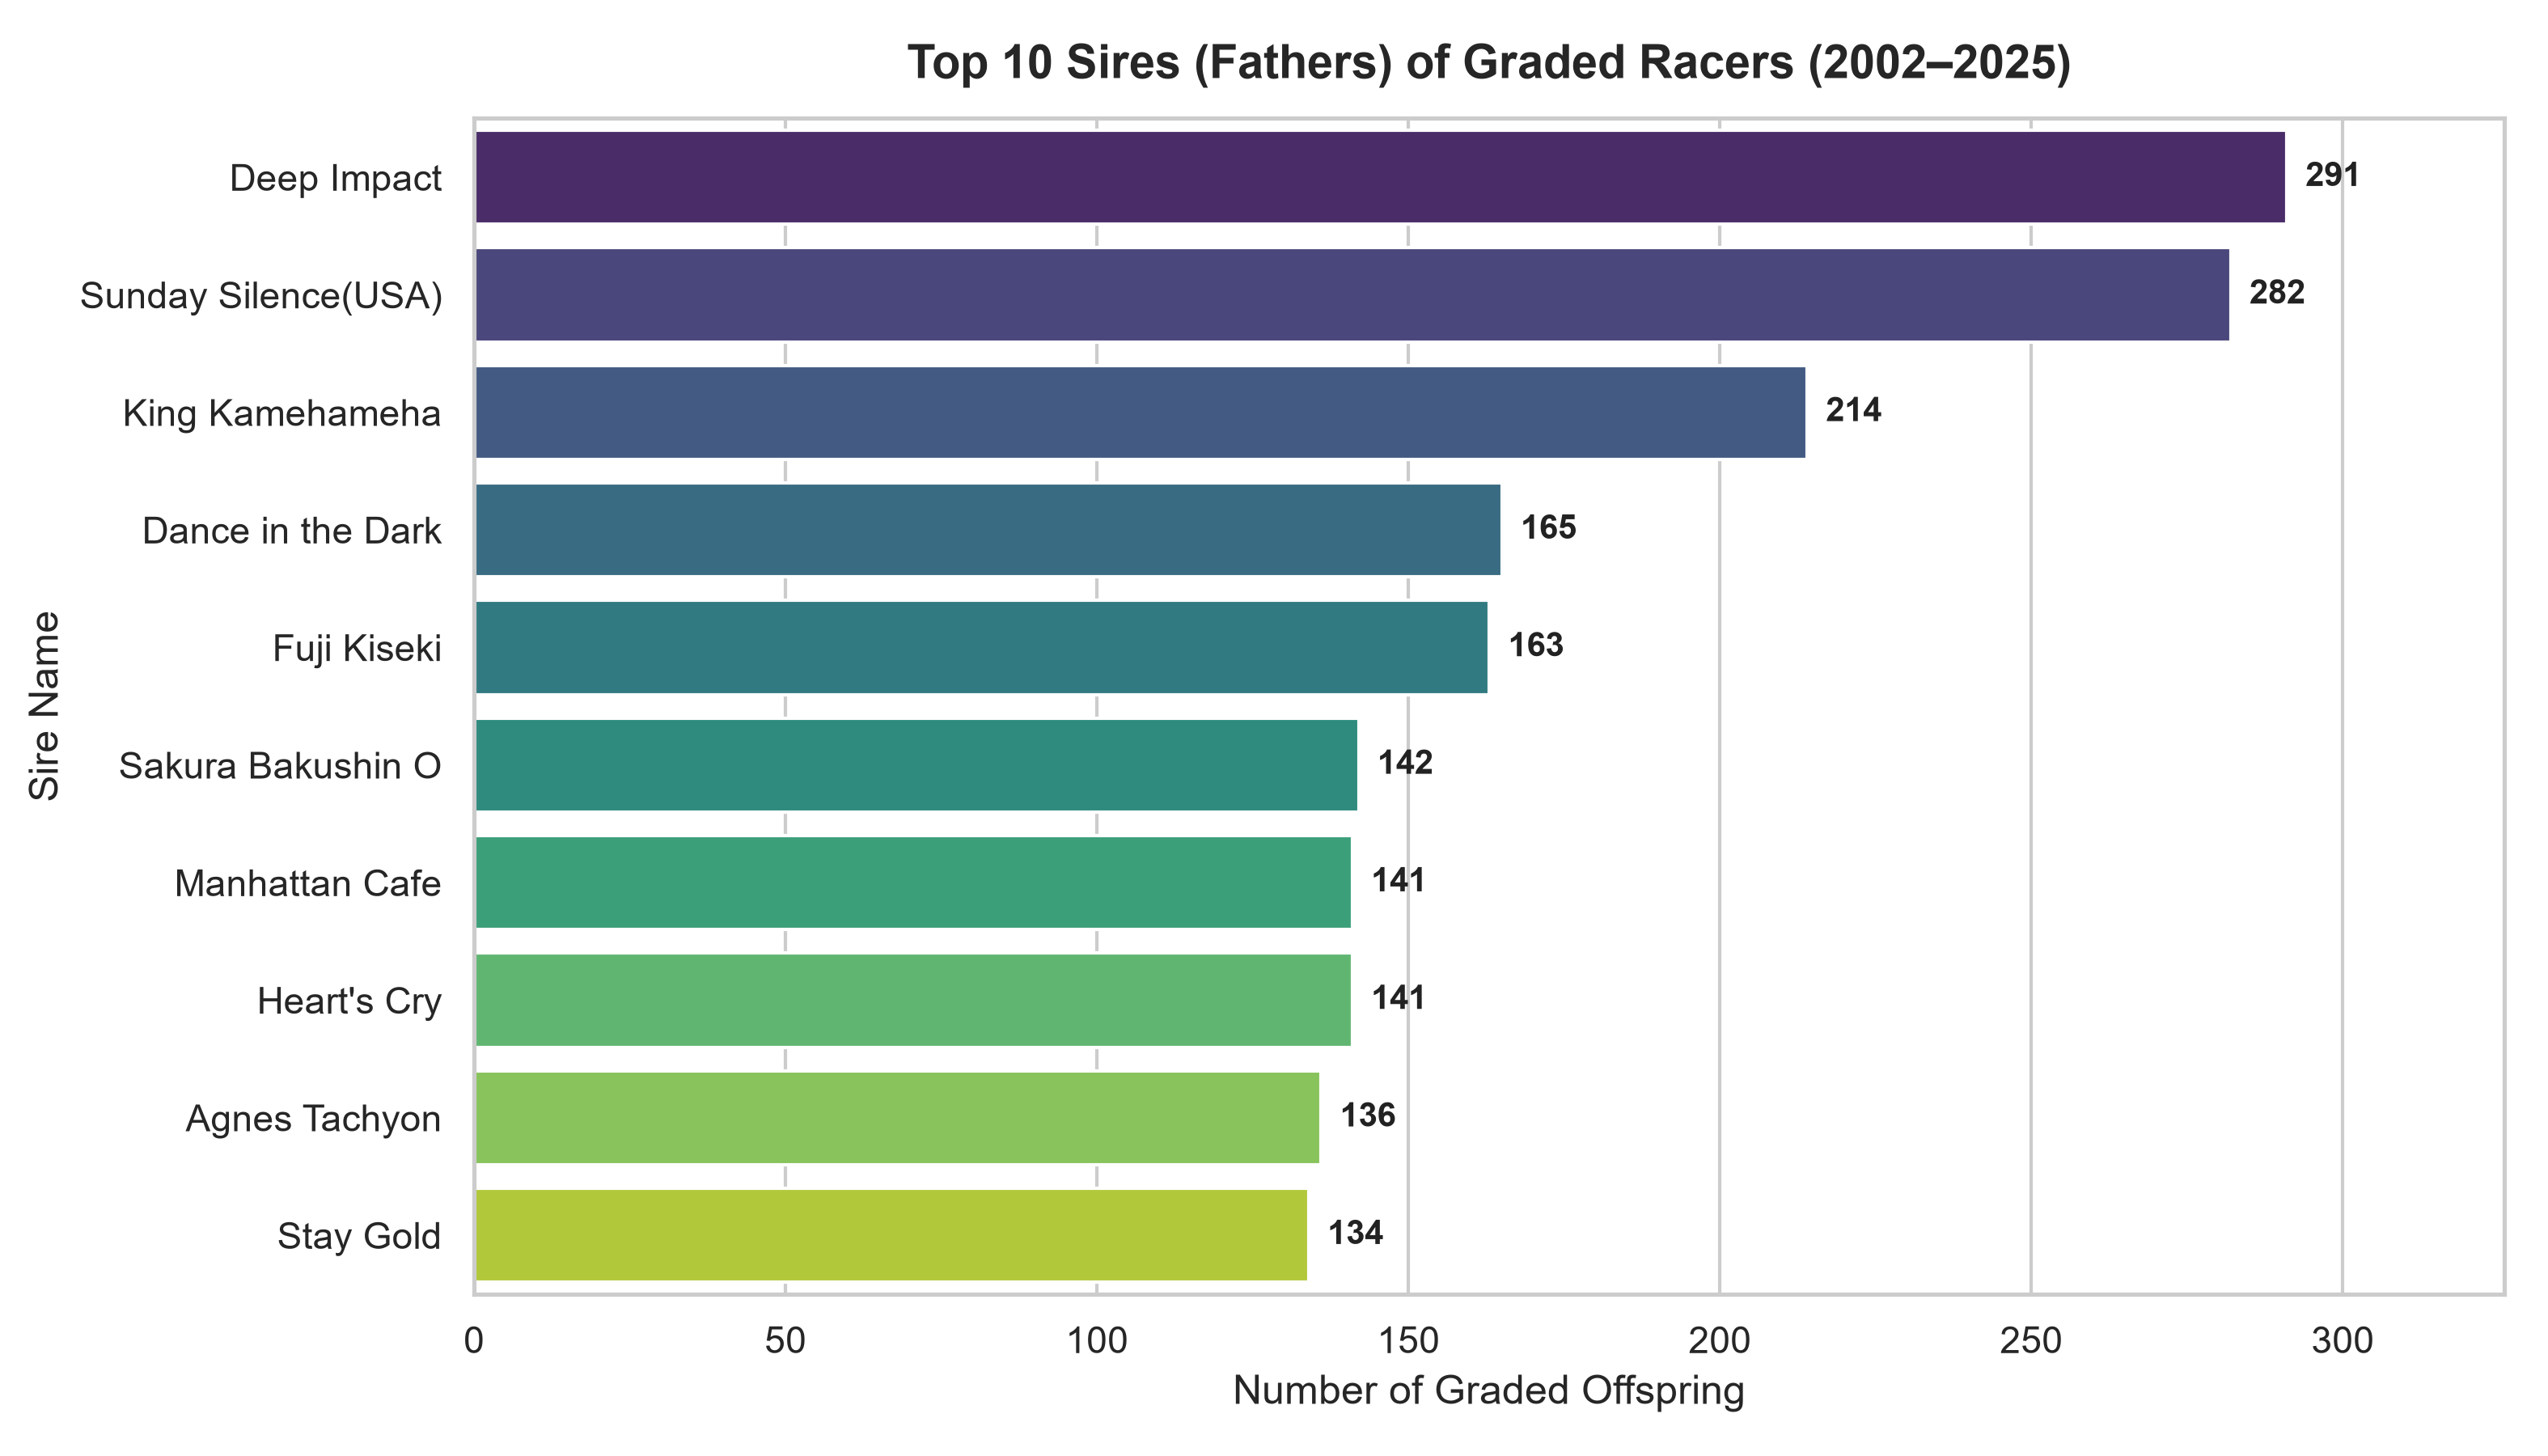
\includegraphics[width=0.98\columnwidth]{../assets/top_sires.png}}
\vspace{2mm}
\centerline{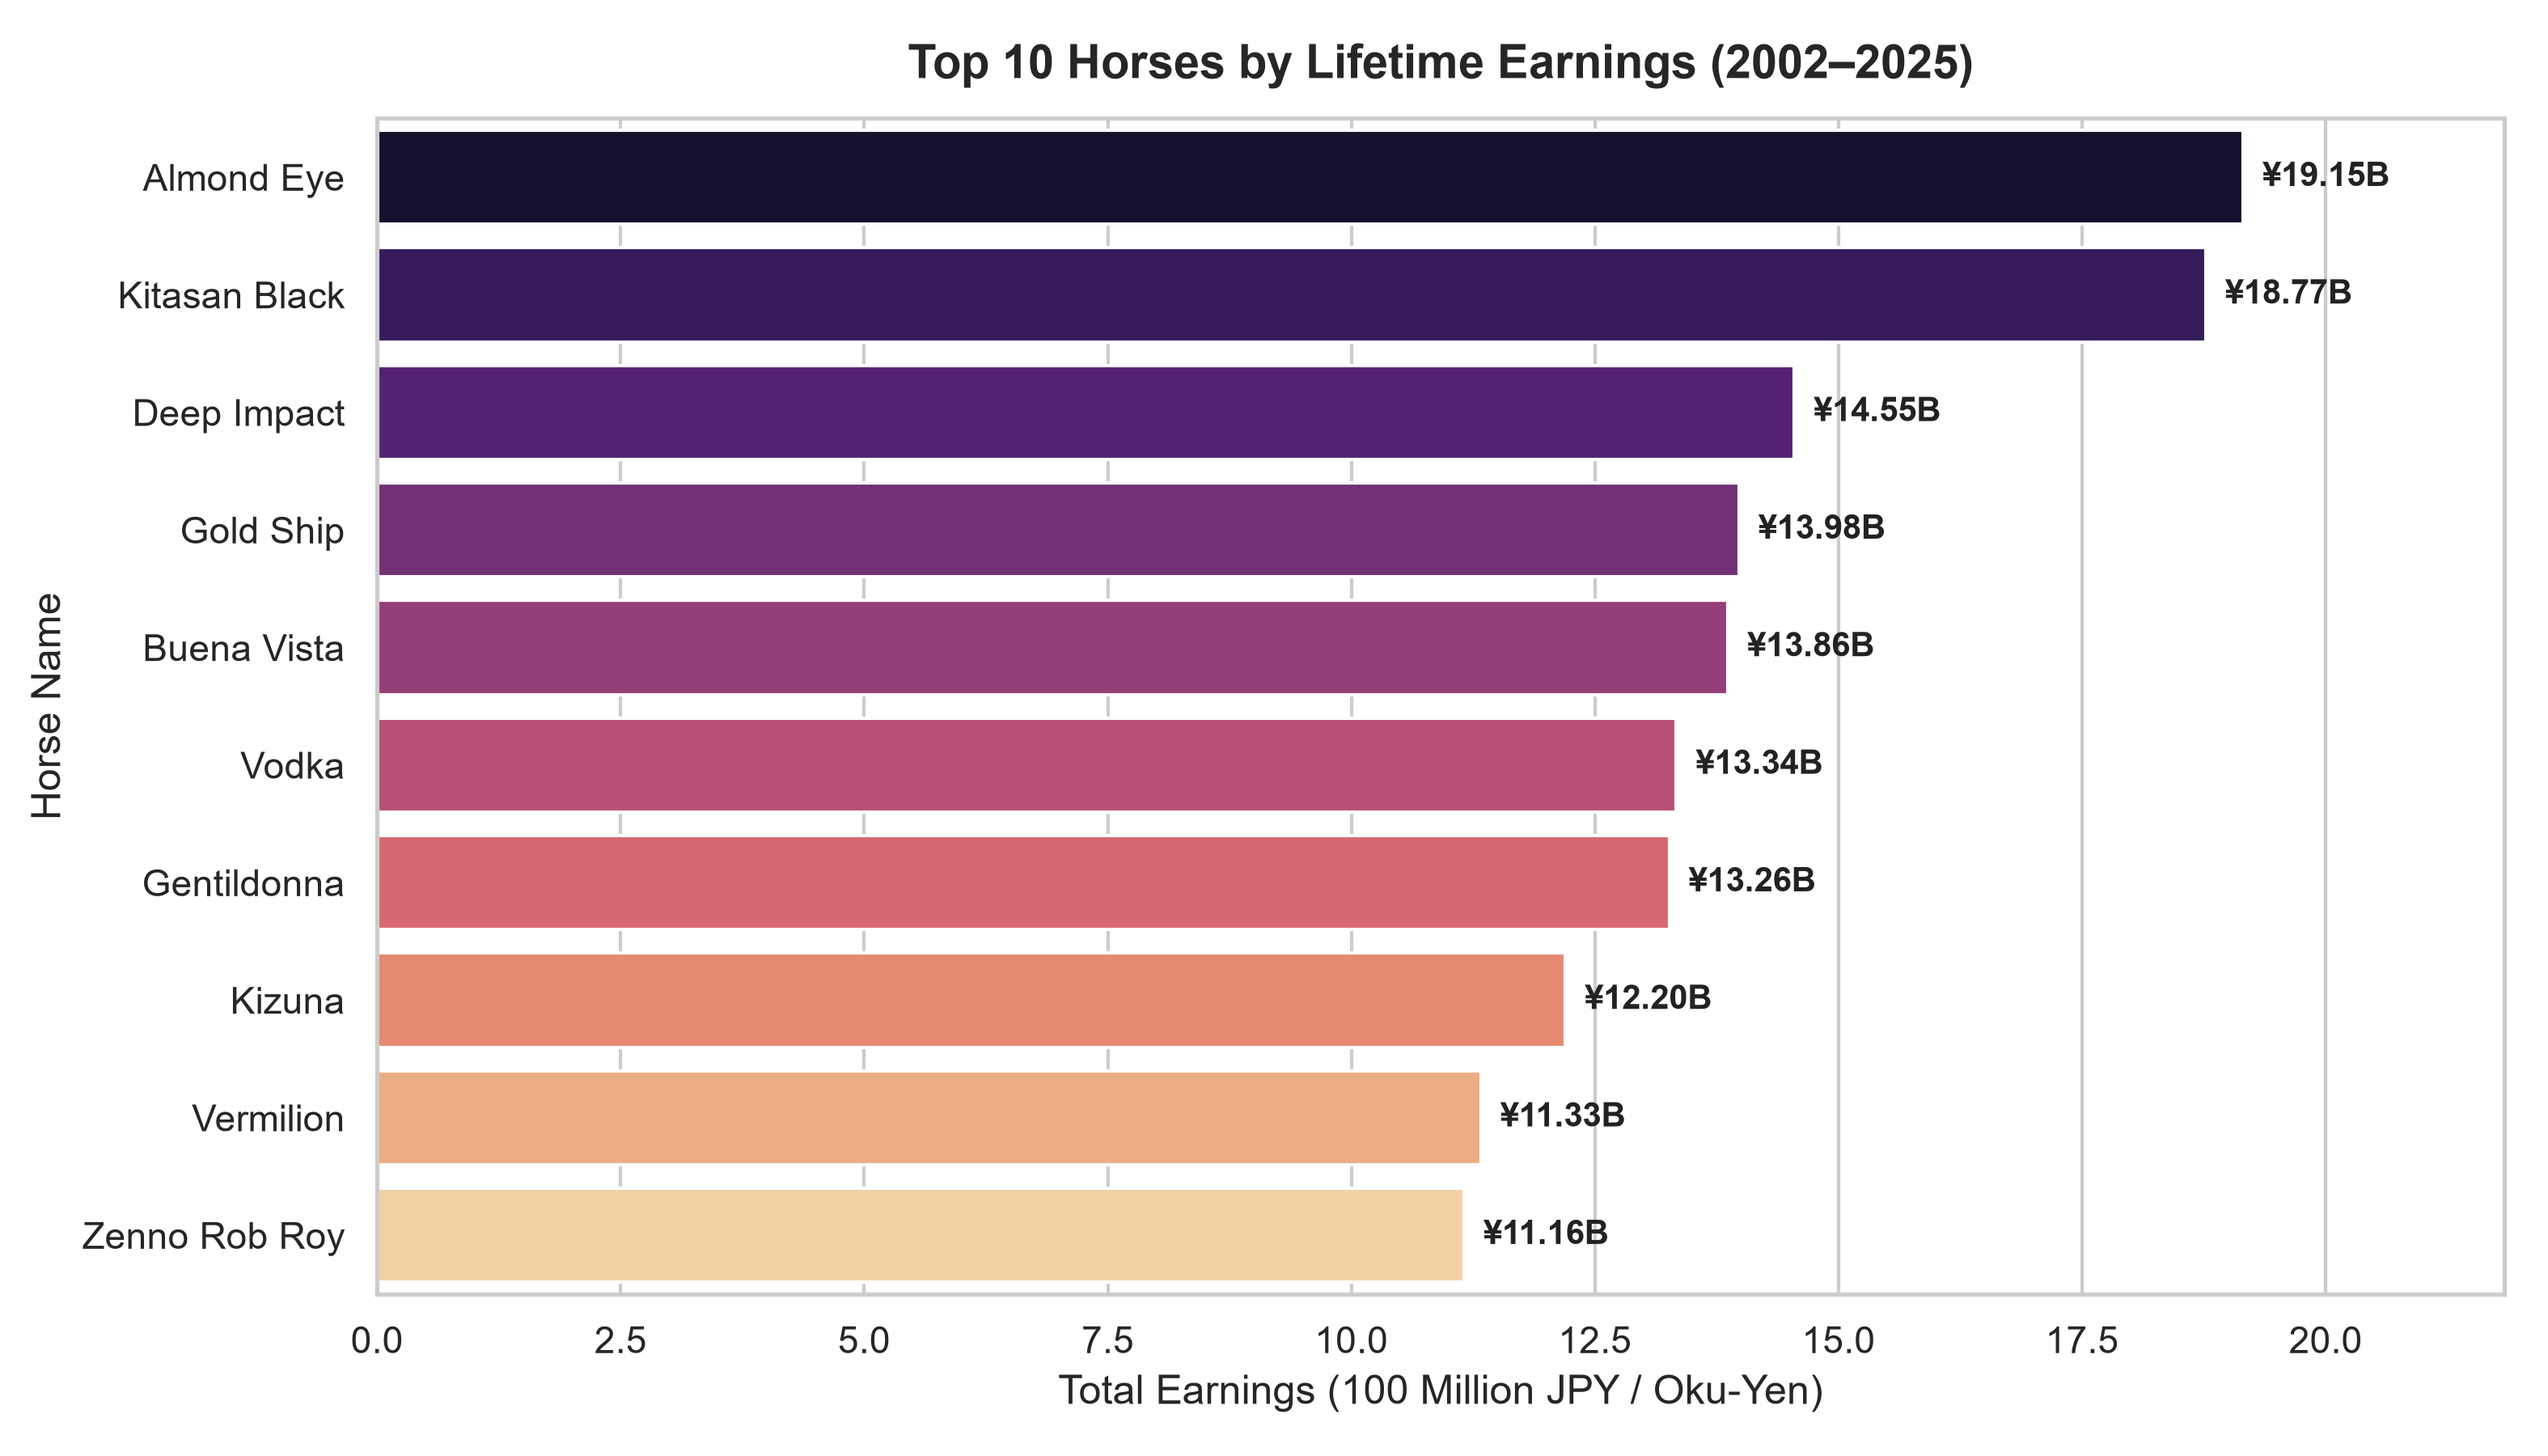
\includegraphics[width=0.98\columnwidth]{../assets/top_earners.png}}
\caption{Acima: Top 10 garanhões (\textit{Sires}) por prole em provas Graded (2002--2025). Abaixo: Top 10 cavalos por premiação acumulada na carreira (em 100 milhões de ienes / \textit{Oku-Yen}).}
\label{fig:top_sires_earners}
\end{figure}

Para superar a limitação unidimensional dos gráficos de barras, construiu-se o \textbf{Diagrama de Fluxo Aluvial / Sankey de 4 Estágios} (Fig.~2), que mapeia simultaneamente $N = 8.857$ participações através dos eixos: \textit{1. Linhagem Paterna} $\to$ \textit{2. Superfície da Pista} $\to$ \textit{3. Regime de Distância} $\to$ \textit{4. Grau da Prova (G1/G2/G3)}. A análise visual do diagrama revela imediatamente a canalização genética das linhagens: enquanto as faixas roxas e azuis de \textit{Deep Impact}, \textit{Sunday Silence} e \textit{King Kamehameha} fluem massivamente para a pista de Grama (\textit{Turf}, 92,6\%
do fluxo das top 10 linhagens) e se concentram nas distâncias intermediárias clássicas ($1800\text{--}2200\text{m}$, 45,6\%),
as fitas laranjas de \textbf{Gold Allure} e \textbf{Brian's Time} desviam fortemente para a pista de Areia (\textit{Dirt}, 7,4\%),
e a faixa azul-clara de \textbf{Sakura Bakushin O} escoa quase integralmente para o regime de velocidade pura (\textit{Sprint} $\le 1400\text{m}$, 17,4\%).

\begin{figure*}[htbp]
\centerline{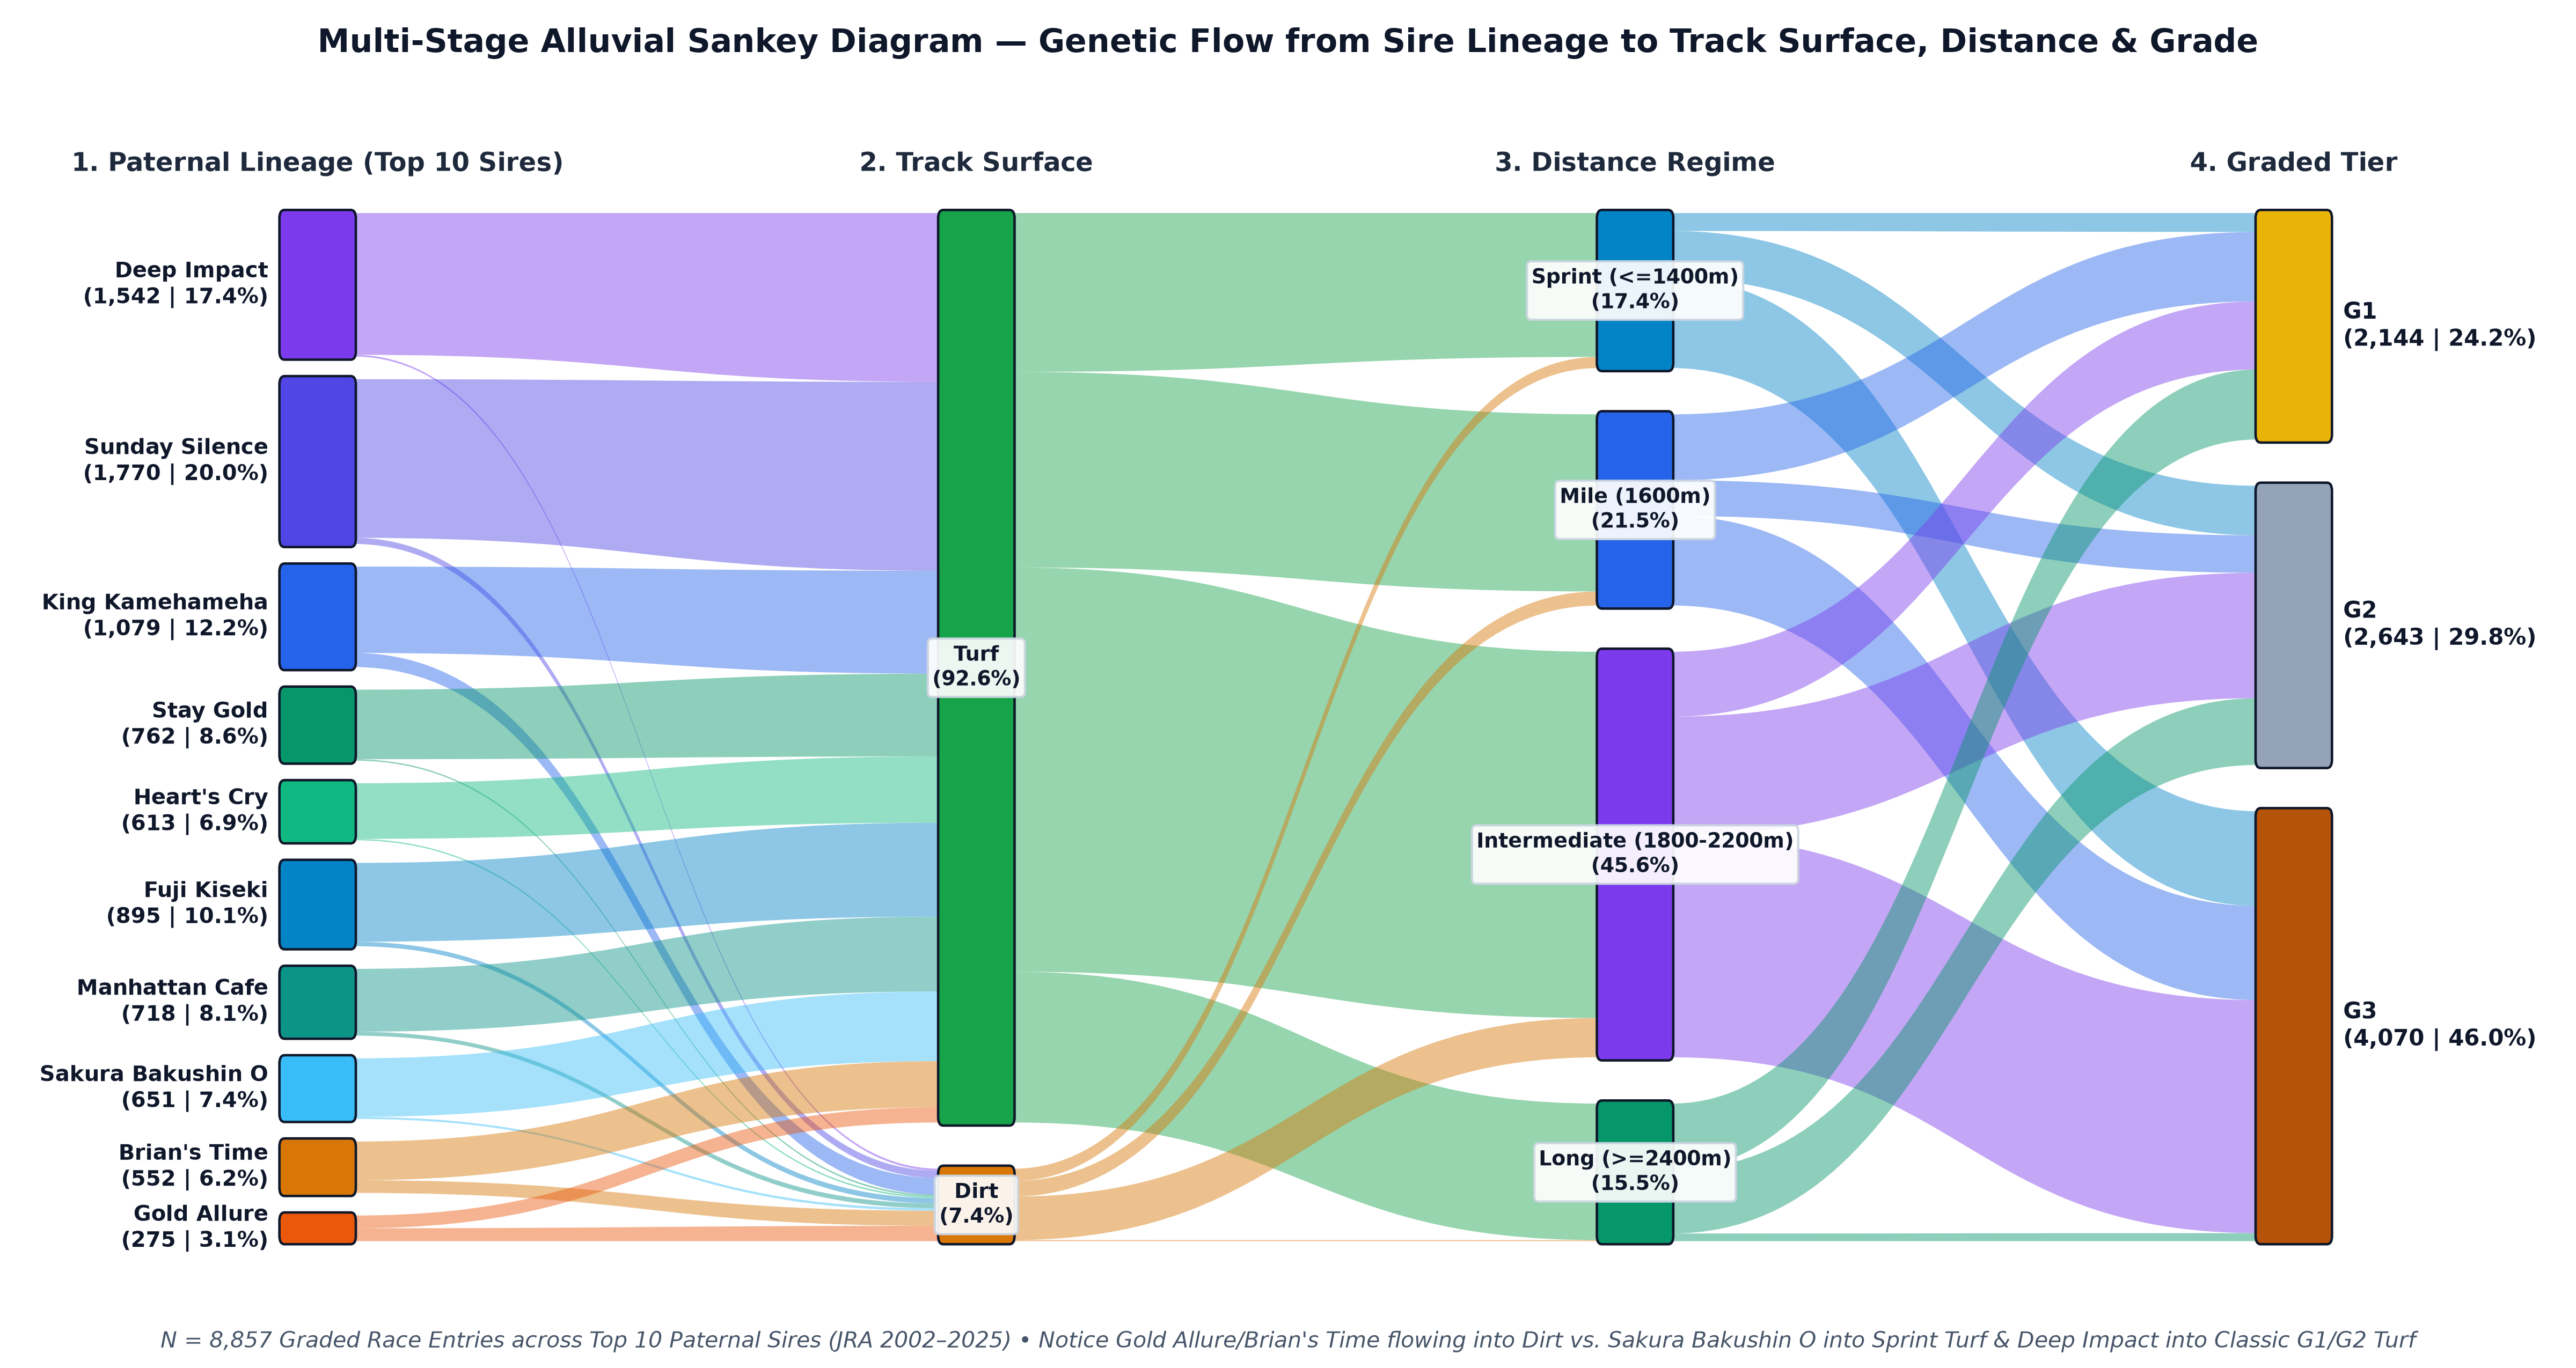
\includegraphics[width=0.95\textwidth]{../assets/superset_alluvial_sankey_flow.png}}
\caption{Diagrama de Fluxo Aluvial / Sankey de 4 Estágios (\textit{Estilo Apache Superset / DataViz Project}): Fluxo genético dos Top 10 Garanhões para Superfície, Regime de Distância e Grau da Corrida ($N = 8.857$ participações).}
\label{fig:sankey}
\end{figure*}

\subsection{Validação do PageRank ($H_2$), Radar Multidimensional e Sunburst dos Hipódromos}
A aplicação do algoritmo PageRank ($d = 0,85$) sobre os 8.135 competidores apresentou forte correlação positiva com o total de pódios Graded na carreira ($r = 0,8799$ de Pearson; $\rho = 0,7597$ de Spearman) e com a premiação acumulada ($r = 0,6266$), confirmando lendas de G1 no topo global (\textit{Kitasan Black}, \textit{Al Ain}, \textit{Vodka}, \textit{Cheval Grand}, \textit{Gold Ship}, \textit{Daiwa Major}, \textit{Buena Vista} e \textit{Gentildonna}). Mais importante, o PageRank validou empiricamente nossa hipótese $H_2$ ao descobrir duas classes de outliers de altíssimo nível competitivo invisíveis à contagem simples de vitórias (Tabela~II):
\begin{enumerate}
    \item \textbf{``Diamantes Injustiçados'' (Zero Vitórias Graded na Carreira):} O cavalo \textbf{\textit{Sounds of Earth}} alcançou a extraordinária \textbf{32ª posição geral entre 8.135 cavalos (Top 0,4\%
da história da JRA)} mesmo possuindo \textbf{zero vitórias} em corridas Graded (0 em 22 largadas no recorte, acumulando 7 pódios de elite, incluindo vice-campeonatos no Kikuka Sho G1, Arima Kinen G1 e Japan Cup G1 contra os maiores campeões da década). De forma análoga, \textbf{\textit{Etariou}} ocupa a \textbf{43ª posição geral} e \textbf{\textit{Fiero}} a \textbf{82ª posição geral} com zero vitórias Graded.
    \item \textbf{``Colecionadores de Prata'' (Zero Vitórias em G1, mas Topo do PageRank):} Competidores como \textbf{\textit{Stephanos}} (\#19 geral), \textbf{\textit{Danburite}} (\#23), \textbf{\textit{Cosmo Bulk}} (\#27), \textbf{\textit{Smart Layer}} (\#31), \textbf{\textit{Real Steel}} (\#33) e \textbf{\textit{Win Variation}} (\#35), que acumularam múltiplos pódios em provas de Grau 1 sem jamais conquistar o troféu principal de G1 na carreira.
\end{enumerate}

\begin{table}[htbp]
\caption{Anomalias Descobertas pelo PageRank Esportivo: ``Diamantes Injustiçados'' (0 Vitórias Graded) e ``Colecionadores de Prata'' (0 Vitórias G1)}
\begin{center}
\renewcommand{\arraystretch}{1.12}
\setlength{\tabcolsep}{3.5pt}
\resizebox{\columnwidth}{!}{%
\begin{tabular}{clcccc}
\toprule
\textbf{Rank PR} & \textbf{Cavalo (\textit{Sire})} & \textbf{PR Esc.} & \textbf{Vit. / G1} & \textbf{Pódios} & \textbf{Ganhos} \\
\midrule
\#19 & Stephanos (\textit{Deep Impact}) & 17,58 & 1 / 0 & 8 & ¥344,6M \\
\#27 & Cosmo Bulk (\textit{Zagreb}) & 16,73 & 3 / 0 & 6 & ¥482,2M \\
\textbf{\#32} & \textbf{Sounds of Earth (\textit{Neo Universe})} & \textbf{16,31} & \textbf{0 / 0} & \textbf{7} & \textbf{¥467,4M} \\
\#33 & Real Steel (\textit{Deep Impact}) & 16,13 & 2 / 0 & 8 & ¥416,8M \\
\#35 & Win Variation (\textit{Heart's Cry}) & 15,78 & 2 / 0 & 11 & ¥579,4M* \\
\textbf{\#43} & \textbf{Etariou (\textit{Stay Gold})} & \textbf{14,89} & \textbf{0 / 0} & \textbf{3} & \textbf{¥238,0M*} \\
\textbf{\#82} & \textbf{Fiero (\textit{Deep Impact})} & \textbf{12,52} & \textbf{0 / 0} & \textbf{9} & \textbf{¥314,5M} \\
\bottomrule
\end{tabular}%
}
\label{tab:pagerank_anomalies}
\end{center}
\end{table}

A Fig.~3 (esquerda) ilustra essa descoberta através de um \textbf{Gráfico Radar Hexagonal}: enquanto \textit{Deep Impact}, \textit{Almond Eye} e \textit{Lord Kanaloa} expandem seus polígonos para 90--100\%
no vértice de \textit{Graded Win Rate}, o polígono tracejado laranja de \textbf{\textit{Sounds of Earth}} colapsa exatamente a 0\%
no vértice de vitórias, mas projeta ampla área nos eixos de \textit{PageRank Prestige}, \textit{G1 Rivalry Volume} e \textit{Stamina Index}. À direita na Fig.~3, o \textbf{Gráfico Sunburst Hierárquico de 3 Anéis} mapeia a distribuição estrutural das 3.216 corridas por Superfície (\textit{Turf} 81,9\%,
\textit{Dirt} 10,7\%,
\textit{Obstacle} 7,4\%)
$\to$ Grau (G1, G2, G3) $\to$ 10 Hipódromos da JRA, evidenciando a concentração das provas de Grau 1 nos quatro circuitos metropolitanos principais (\textit{Tokyo}, \textit{Kyoto}, \textit{Hanshin} e \textit{Nakayama}).

\begin{figure*}[htbp]
\centerline{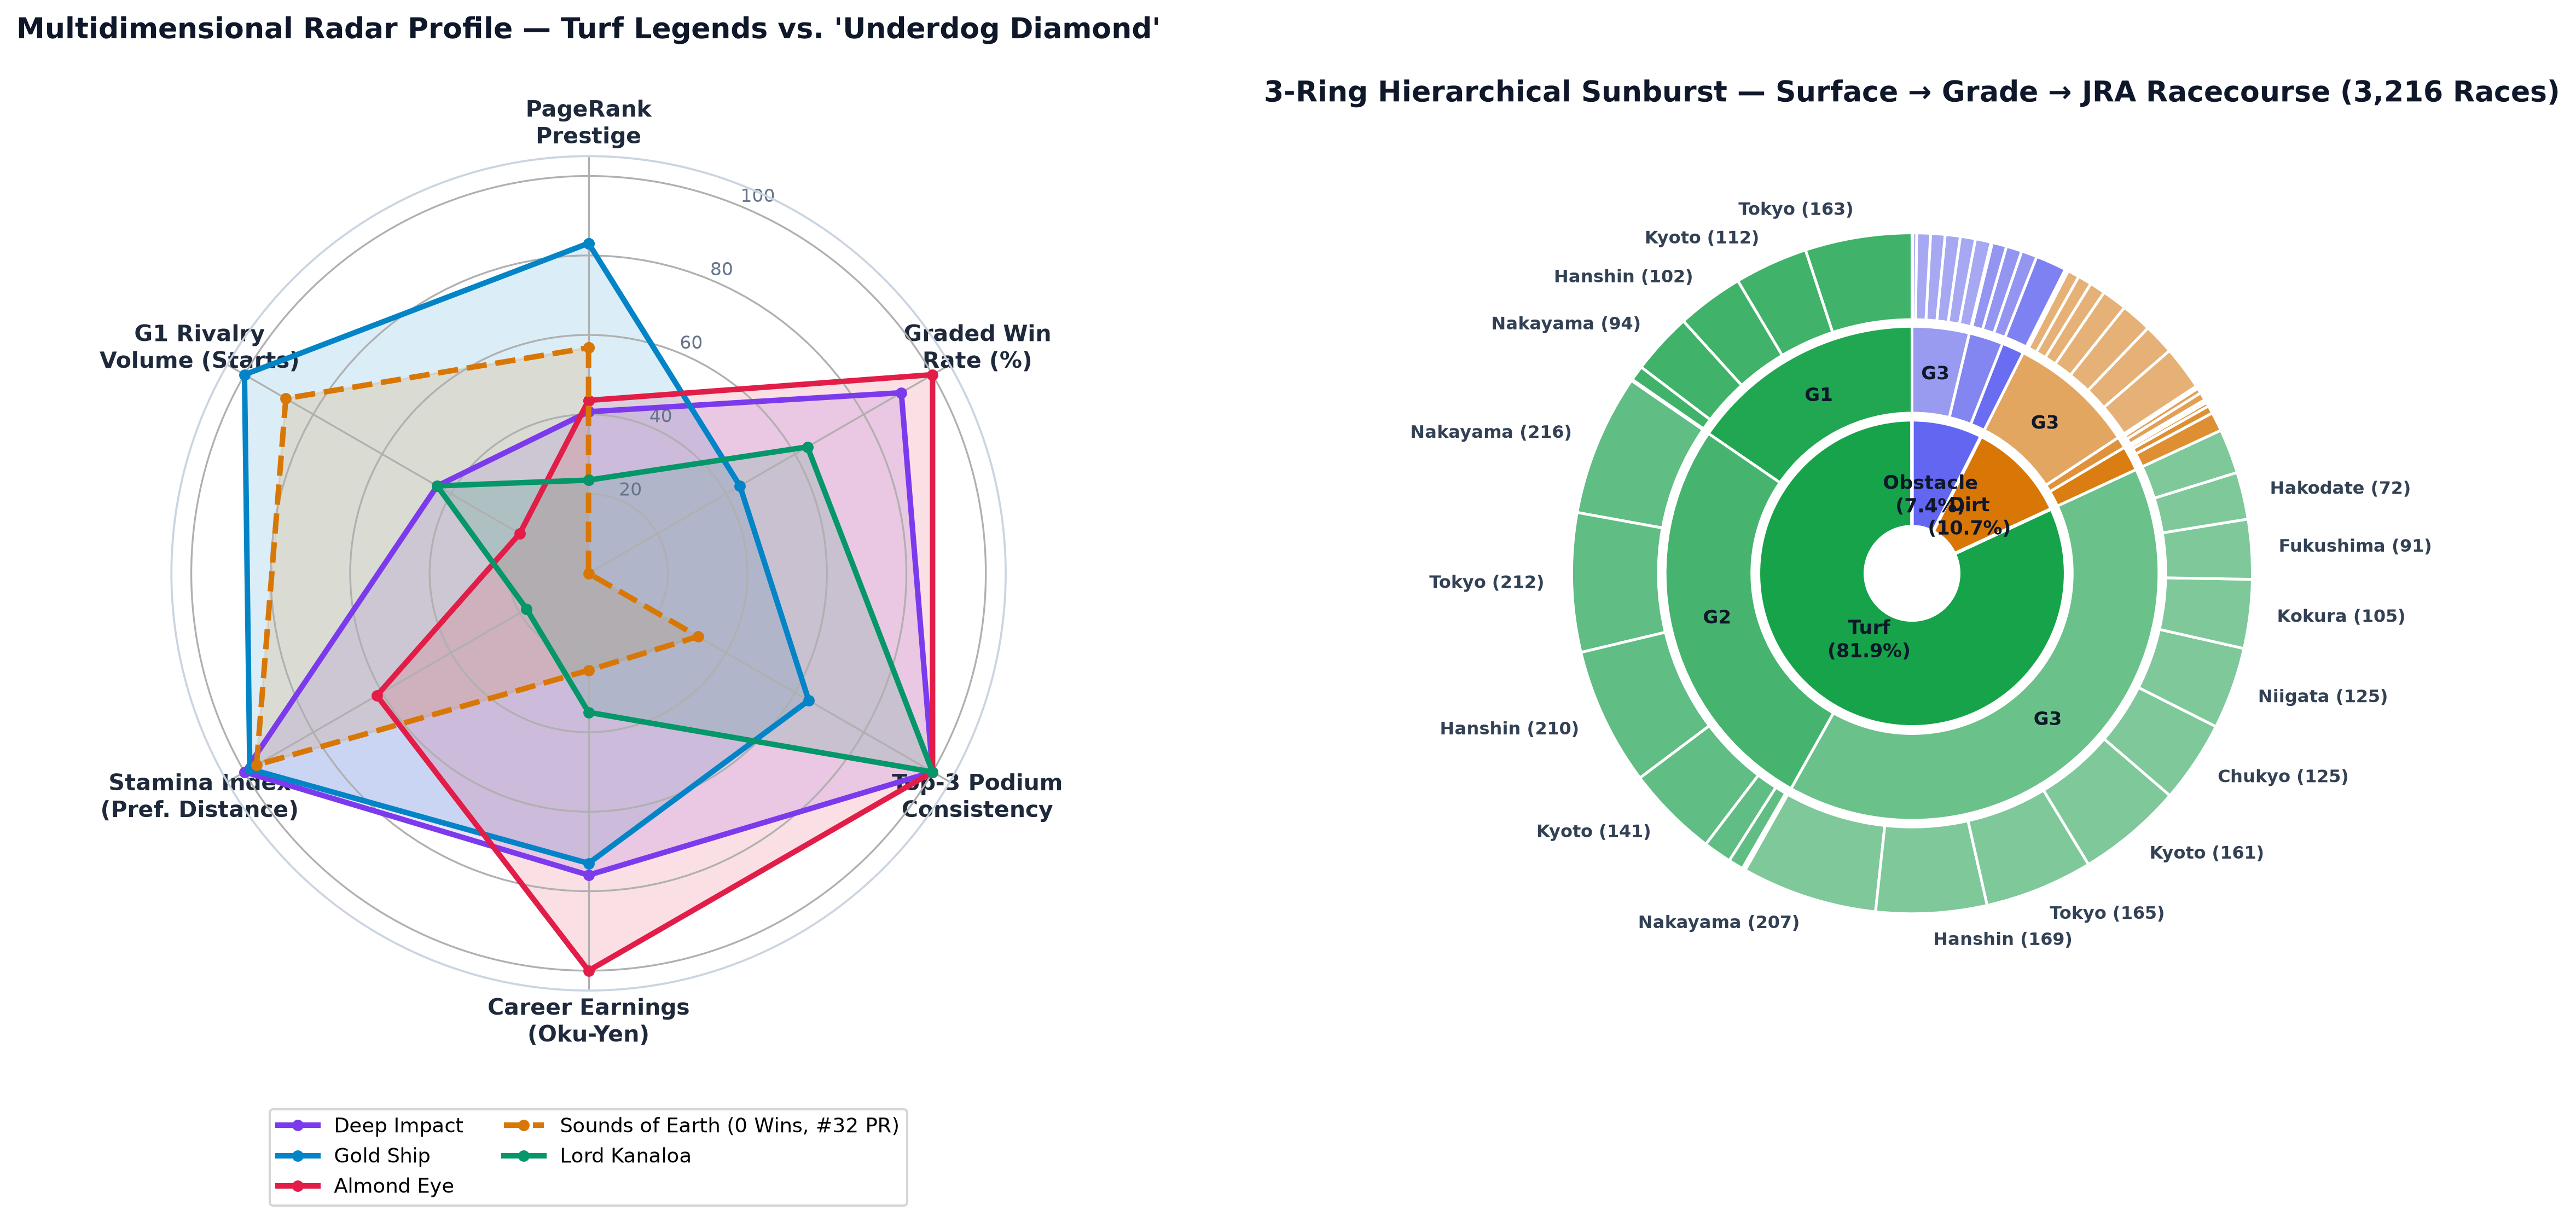
\includegraphics[width=0.95\textwidth]{../assets/superset_radar_and_sunburst.png}}
\caption{Esquerda: Perfil Radar Hexagonal comparando lendas do turfe com o ``Diamante Injustiçado'' \textit{Sounds of Earth} (\#32 PageRank com 0 vitórias). Direita: Sunburst Hierárquico de 3 Anéis (\textit{Superfície $\to$ Grau $\to$ Hipódromo JRA}) sobre as 3.216 corridas.}
\label{fig:radar_sunburst}
\end{figure*}

\subsection{Sucessão Geracional (Streamgraph), Biometria Equina (Split-Violin) e Especialização Genética ($H_1$)}
O \textbf{Streamgraph Simétrico Temporal} (Fig.~4) revela a dinâmica evolutiva de substituição geracional ao longo das temporadas: a \textbf{Era I (2002--2007)} é dominada pela prole direta de \textit{Sunday Silence} e \textit{Brian's Time}; a \textbf{Era II (2008--2012)} marca a ascensão da primeira geração doméstica (\textit{Fuji Kiseki}, \textit{Dance in the Dark}, \textit{Agnes Tachyon} e \textit{Manhattan Cafe}); e a \textbf{Era III (2013+)} consolida a hegemonia absoluta de \textit{Deep Impact}, acompanhado por \textit{King Kamehameha}, \textit{Stay Gold}, \textit{Heart's Cry}, \textit{Daiwa Major} e \textit{Lord Kanaloa}.

\begin{figure*}[htbp]
\centerline{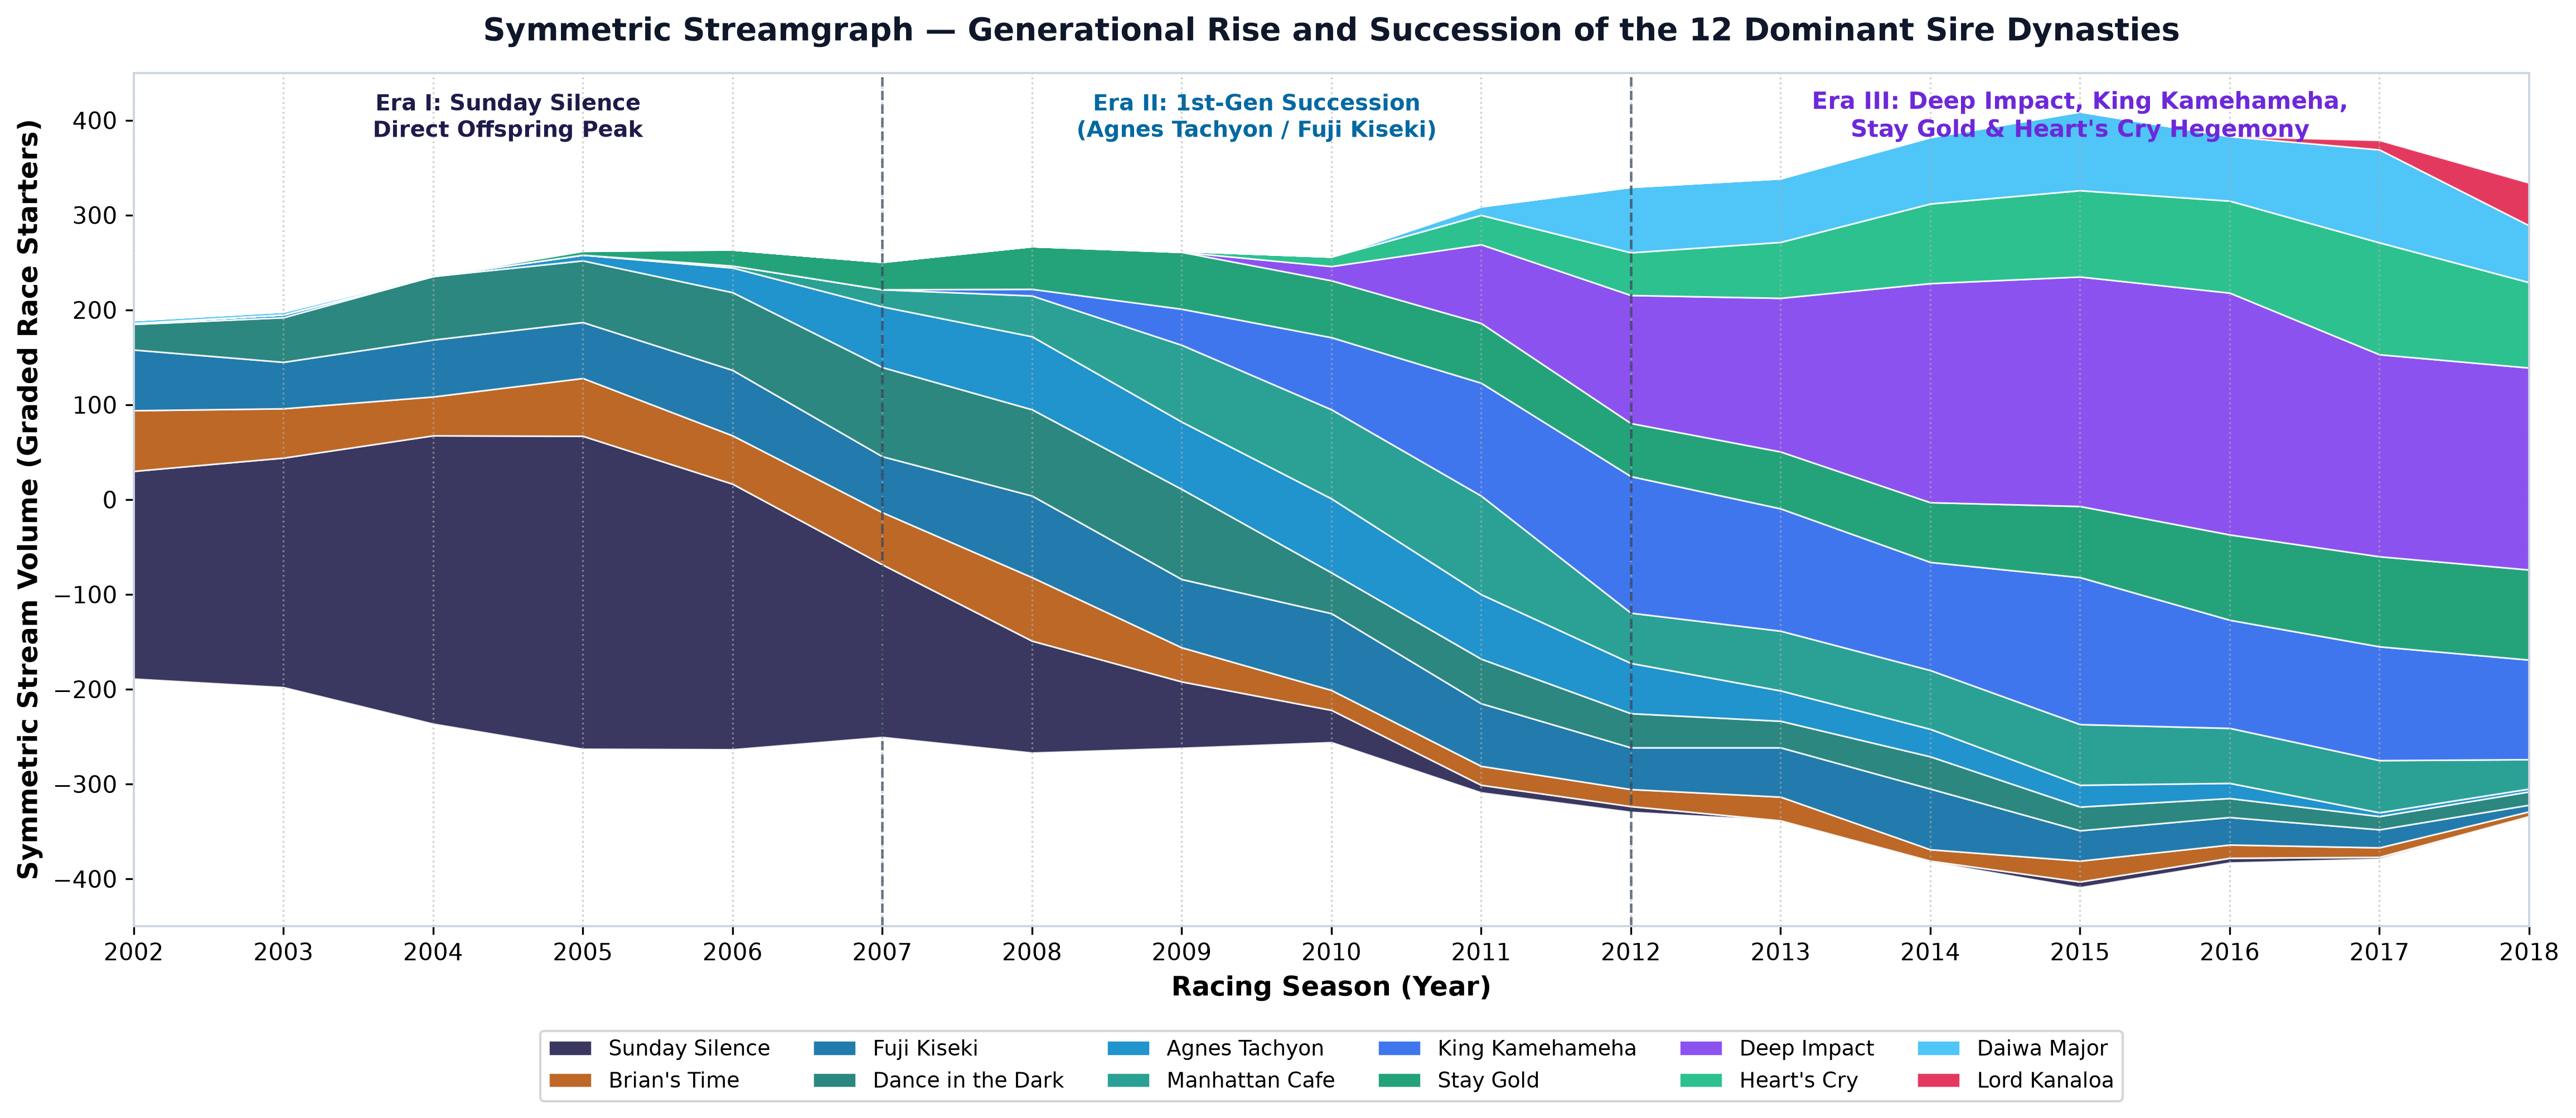
\includegraphics[width=0.92\textwidth]{../assets/superset_streamgraph_dynasties.png}}
\caption{Streamgraph Simétrico Temporal demonstrando a ascensão e sucessão geracional das 12 principais dinastias paternas na JRA.}
\label{fig:streamgraph}
\end{figure*}

A análise biométrica através do gráfico \textbf{Split-Violin} (Fig.~5, esquerda) sobre a massa corporal dos animais no dia da corrida (\texttt{horse\_mass\_kg}) revelou um dimorfismo físico marcante e estatisticamente consistente em todos os quatro regimes de distância: cavalos que competem na \textbf{Areia (\textit{Dirt}, metade laranja)} apresentam massa corporal média entre \textbf{494,0 kg e 498,2 kg}, sendo cerca de \textbf{16 kg a 21 kg mais pesados e musculosos} do que os competidores de \textbf{Grama (\textit{Turf}, metade verde, média entre 473,0 kg e 482,4 kg)}. Fisicamente, pistas de areia exigem maior potência muscular e tração mecânica, enquanto pistas de grama favorecem uma maior relação peso-potência e economia elástica de passadas.

\begin{figure*}[htbp]
\centerline{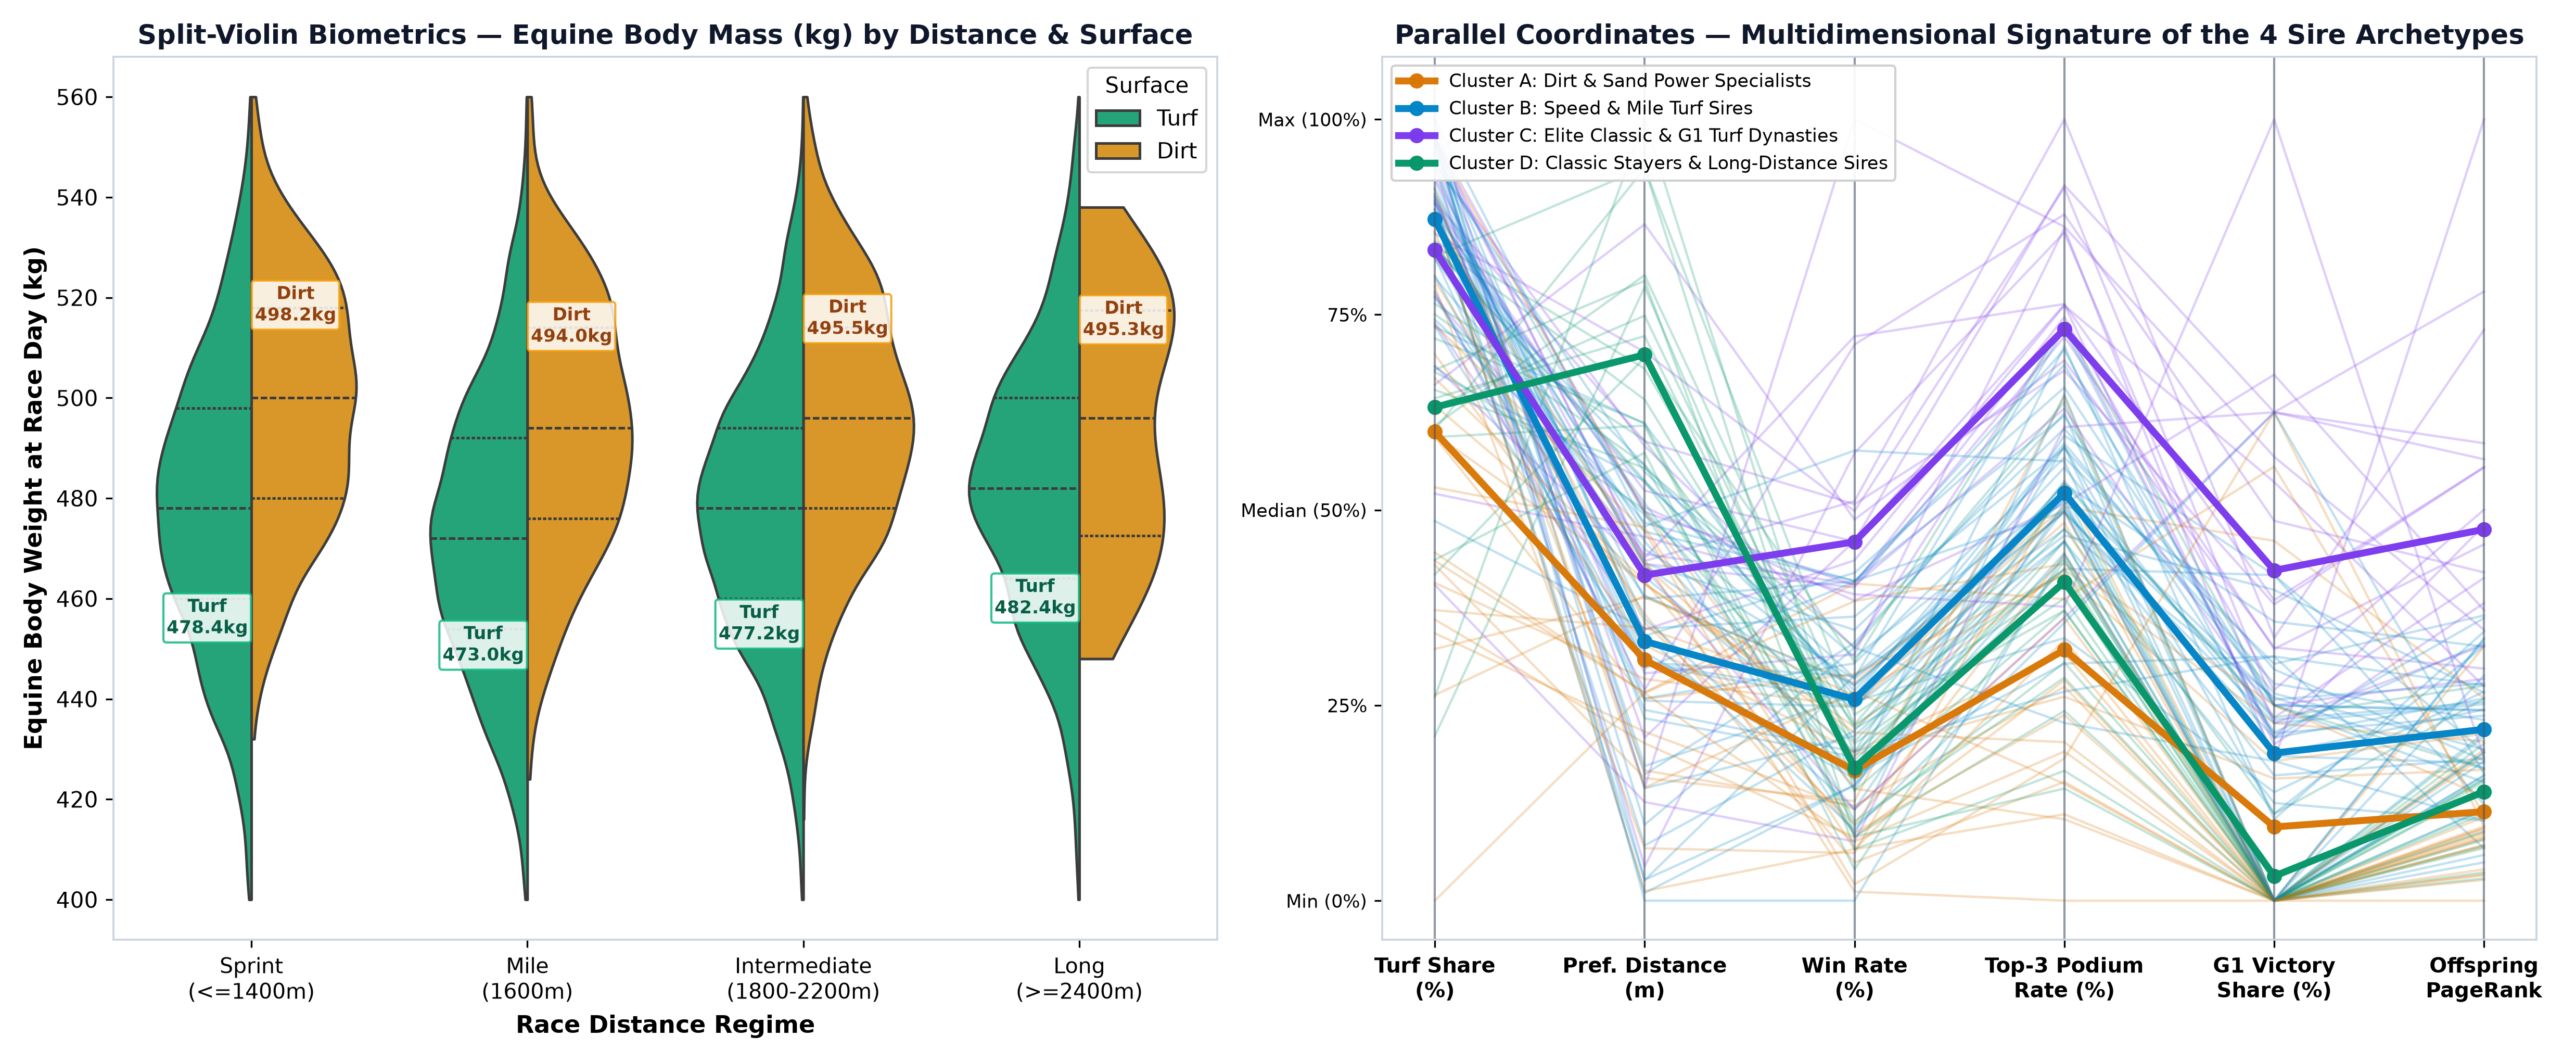
\includegraphics[width=0.95\textwidth]{../assets/superset_raincloud_and_parallel.png}}
\caption{Esquerda: Distribuição Split-Violin da massa corporal equina (kg) por regime de distância e superfície (\textit{Turf} vs. \textit{Dirt}). Direita: Coordenadas Paralelas traçando a assinatura multidimensional dos 4 arquétipos de garanhões.}
\label{fig:violin_parallel}
\end{figure*}

Nos testes formais de hipóteses para $H_1$ (\path{src/ml_analysis.py}), o teste Qui-Quadrado de independência entre os Top 15 garanhões e a superfície rejeitou a hipótese nula com significância extrema ($\chi^2 = 739,99, gl = 14, p = 2,43 \times 10^{-107}, V \text{ de Cramér} = 0,2514$). Na distribuição por categoria de distância (Fig.~7, direita), obteve-se $\chi^2 = 2237,47$ ($gl = 42, p = 3,71 \times 10^{-317}, V = 0,2523$): enquanto \textit{Sakura Bakushin O} concentra 64,6\%
das largadas de seus filhos em provas de \textit{Sprint} ($\le 1400\text{m}$), \textit{Stay Gold} (78,1\%
$\ge 1800\text{m}$), \textit{Heart's Cry} (78,9\%
$\ge 1800\text{m}$) e \textit{Dance in the Dark} (32,4\%
$\ge 2400\text{m}$) transmitem estamina clássica e de fundo. A ANOVA One-Way ($F(14, 930) = 16,46, \eta^2 = 0,1986, p = 1,68 \times 10^{-35}$) e o teste de Kruskal-Wallis ($H = 192,40, p = 2,02 \times 10^{-29}$) confirmam que quase 20\%
da variância total da distância de vitória deve-se diretamente ao pai imediato. Adicionalmente, a avaliação do Coeficiente de Endogamia de Wright ($F_X$) nos 504.074 nós genealógicos comprovou que \textbf{\textit{Northern Dancer (CAN)}} é o principal patriarca de endocruzamento (presente como ancestral comum LCA em 4.206 cavalos endogâmicos que somam 1.211 vitórias Graded), seguido por \textit{Hail to Reason (USA)} (891 cavalos, 256 vitórias) e \textit{Nasrullah (GB)} (631 cavalos, 159 vitórias).

\subsection{Clusterização Não-Supervisionada (K-Means++ PCA) e Predição Supervisionada (Random Forest)}
A Fig.~6 apresenta a projeção dos 106 garanhões nos dois primeiros eixos da Análise de Componentes Principais (\textbf{63,4\%
de variância total explicada}: $\text{PC}_1 = 44,1$\%
capturando o eixo superfície/distância e $\text{PC}_2 = 19,2$\%
capturando a letalidade e prestígio em G1), juntamente com a curva de \textit{Silhouette Score} ($k = 2 \dots 7$). A partição em $k = 4$ isolou quatro arquétipos zootécnicos perfeitamente interpretáveis (também visualizados nas Coordenadas Paralelas da Fig.~5, direita):
\begin{itemize}
    \item \textbf{Cluster A --- \textit{Dirt \& Sand Power Specialists} ($n = 26$):} \textit{Gold Allure}, \textit{Brian's Time}, \textit{Agnes Digital}, \textit{Wild Rush};
    \item \textbf{Cluster B --- \textit{Speed \& Mile Turf Sires} ($n = 41$):} \textit{Sakura Bakushin O}, \textit{Fuji Kiseki}, \textit{Daiwa Major}, \textit{Agnes Tachyon};
    \item \textbf{Cluster C --- \textit{Elite Classic \& G1 Turf Dynasties} ($n = 20$):} \textit{Deep Impact}, \textit{Sunday Silence}, \textit{King Kamehameha}, \textit{Stay Gold}, \textit{Heart's Cry}, \textit{Lord Kanaloa};
    \item \textbf{Cluster D --- \textit{Classic Stayers \& Long-Distance Sires} ($n = 19$):} \textit{Dance in the Dark}, \textit{Mayano Top Gun}, \textit{Marvelous Sunday}.
\end{itemize}

\begin{figure*}[htbp]
\centerline{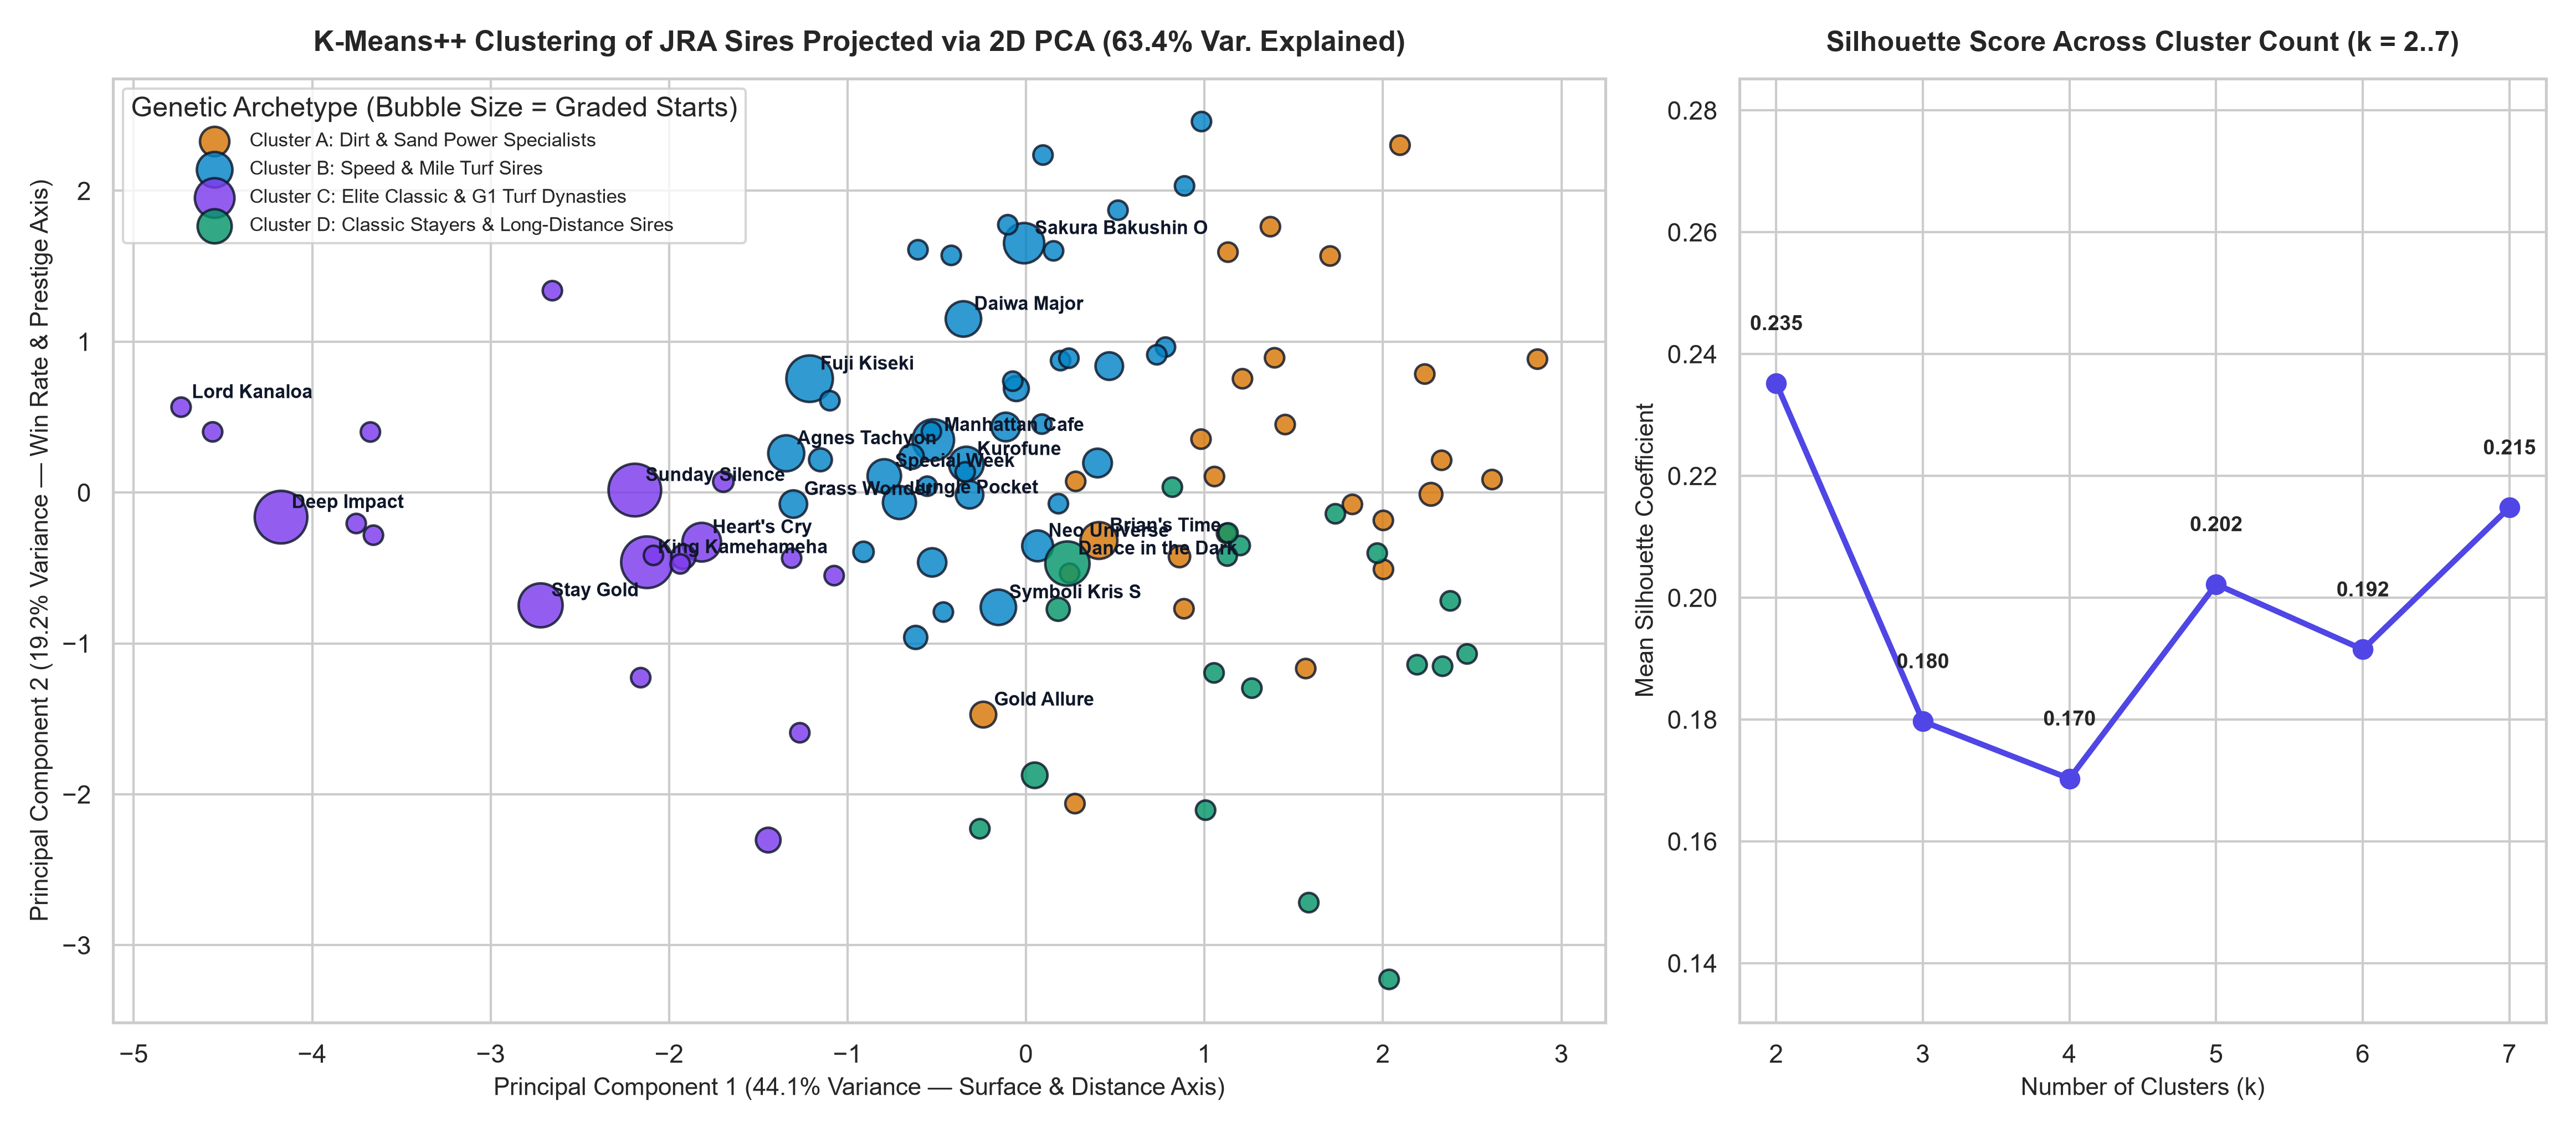
\includegraphics[width=0.94\textwidth]{../assets/ml_kmeans_pca_clusters.png}}
\caption{Esquerda: Clusterização K-Means++ dos 106 garanhões projetada via PCA 2D (63,4\%
de variância explicada). Direita: Curva de Silhouette Score para $k = 2 \dots 7$.}
\label{fig:kmeans_pca}
\end{figure*}

Na tarefa de classificação supervisionada para predição de pódio (\mbox{Top-3}) no conjunto de teste cronológico futuro (\textbf{2016--2018, $N_{\text{teste}} = 5.889$}, Tabela~III), o modelo \textbf{Random Forest (CART Ensemble)} alcançou \textbf{ROC-AUC de 0,7260} (Intervalo de Confiança Bootstrap 95\%:
$[0,7109;\; 0,7389]$), \textbf{PR-AUC de 0,4187} (mais que o dobro do baseline estratificado de $0,2089$) e \textbf{F1-Score de 0,4585}, superando a Regressão Logística L2 ($\text{ROC-AUC} = 0,7144$).

\begin{table}[htbp]
\caption{Desempenho Preditivo de Pódio (\mbox{Top-3}) no Conjunto de Teste Cronológico Out-of-Time (2016--2018, $N = 5.889$)}
\begin{center}
\renewcommand{\arraystretch}{1.15}
\setlength{\tabcolsep}{3.5pt}
\resizebox{\columnwidth}{!}{%
\begin{tabular}{lcccc}
\toprule
\textbf{Modelo Supervisionado} & \textbf{ROC-AUC (IC 95\%)} & \textbf{PR-AUC} & \textbf{F1} & \textbf{Acc.} \\
\midrule
Baseline Estratificado & $0,5000$ (---) & $0,2089$ & $0,0000$ & $0,7911$ \\
Regressão Logística L2 & $0,7144$ ($[0,699;\; 0,728]$) & $\mathbf{0,4257}$ & $0,4413$ & $0,6762$ \\
\textbf{Random Forest (CART)} & $\mathbf{0,7260}$ ($\mathbf{[0,711;\; 0,739]}$) & $0,4187$ & $\mathbf{0,4585}$ & $\mathbf{0,6908}$ \\
\bottomrule
\end{tabular}%
}
\label{tab:ml_results}
\end{center}
\end{table}

A inspeção da Importância Relativa de Gini da Random Forest (Fig.~7, esquerda) responde quantitativamente ao dilema entre genética e fator humano: no momento da largada, a \textbf{taxa histórica prévia de pódios do jóquei (\texttt{jockey\_prior\_top3\_rate}, 29,77\%)}
e o \textbf{retrospecto prévio do próprio cavalo (\texttt{horse\_prior\_top3\_rate}, 22,70\%)}
detêm mais da metade do poder decisório do modelo, seguidos pela idade biológica (\texttt{age}, 9,09\%),
experiência acumulada (\texttt{horse\_prior\_starts}, 5,70\%),
tamanho do grid (\texttt{num\_runners}, 5,10\%),
taxa prévia do treinador (\texttt{trainer\_prior\_top3\_rate}, 4,90\%),
exigência da prova (\texttt{grade\_weight}, 4,28\%)
e afinidade genética do garanhão com a superfície (\texttt{sire\_surface\_affinity}, 3,88\%)
e avô materno (\texttt{damsire\_prior\_top3\_rate}, 2,90\%).
Em síntese: \textit{a herança genética atua como o filtro biológico estrutural que define em qual superfície e distância o animal é competitivo, enquanto a sinergia humana (jóquei/treinador) e a forma atlética recente determinam quem vence o confronto direto}.

\begin{figure*}[htbp]
\centerline{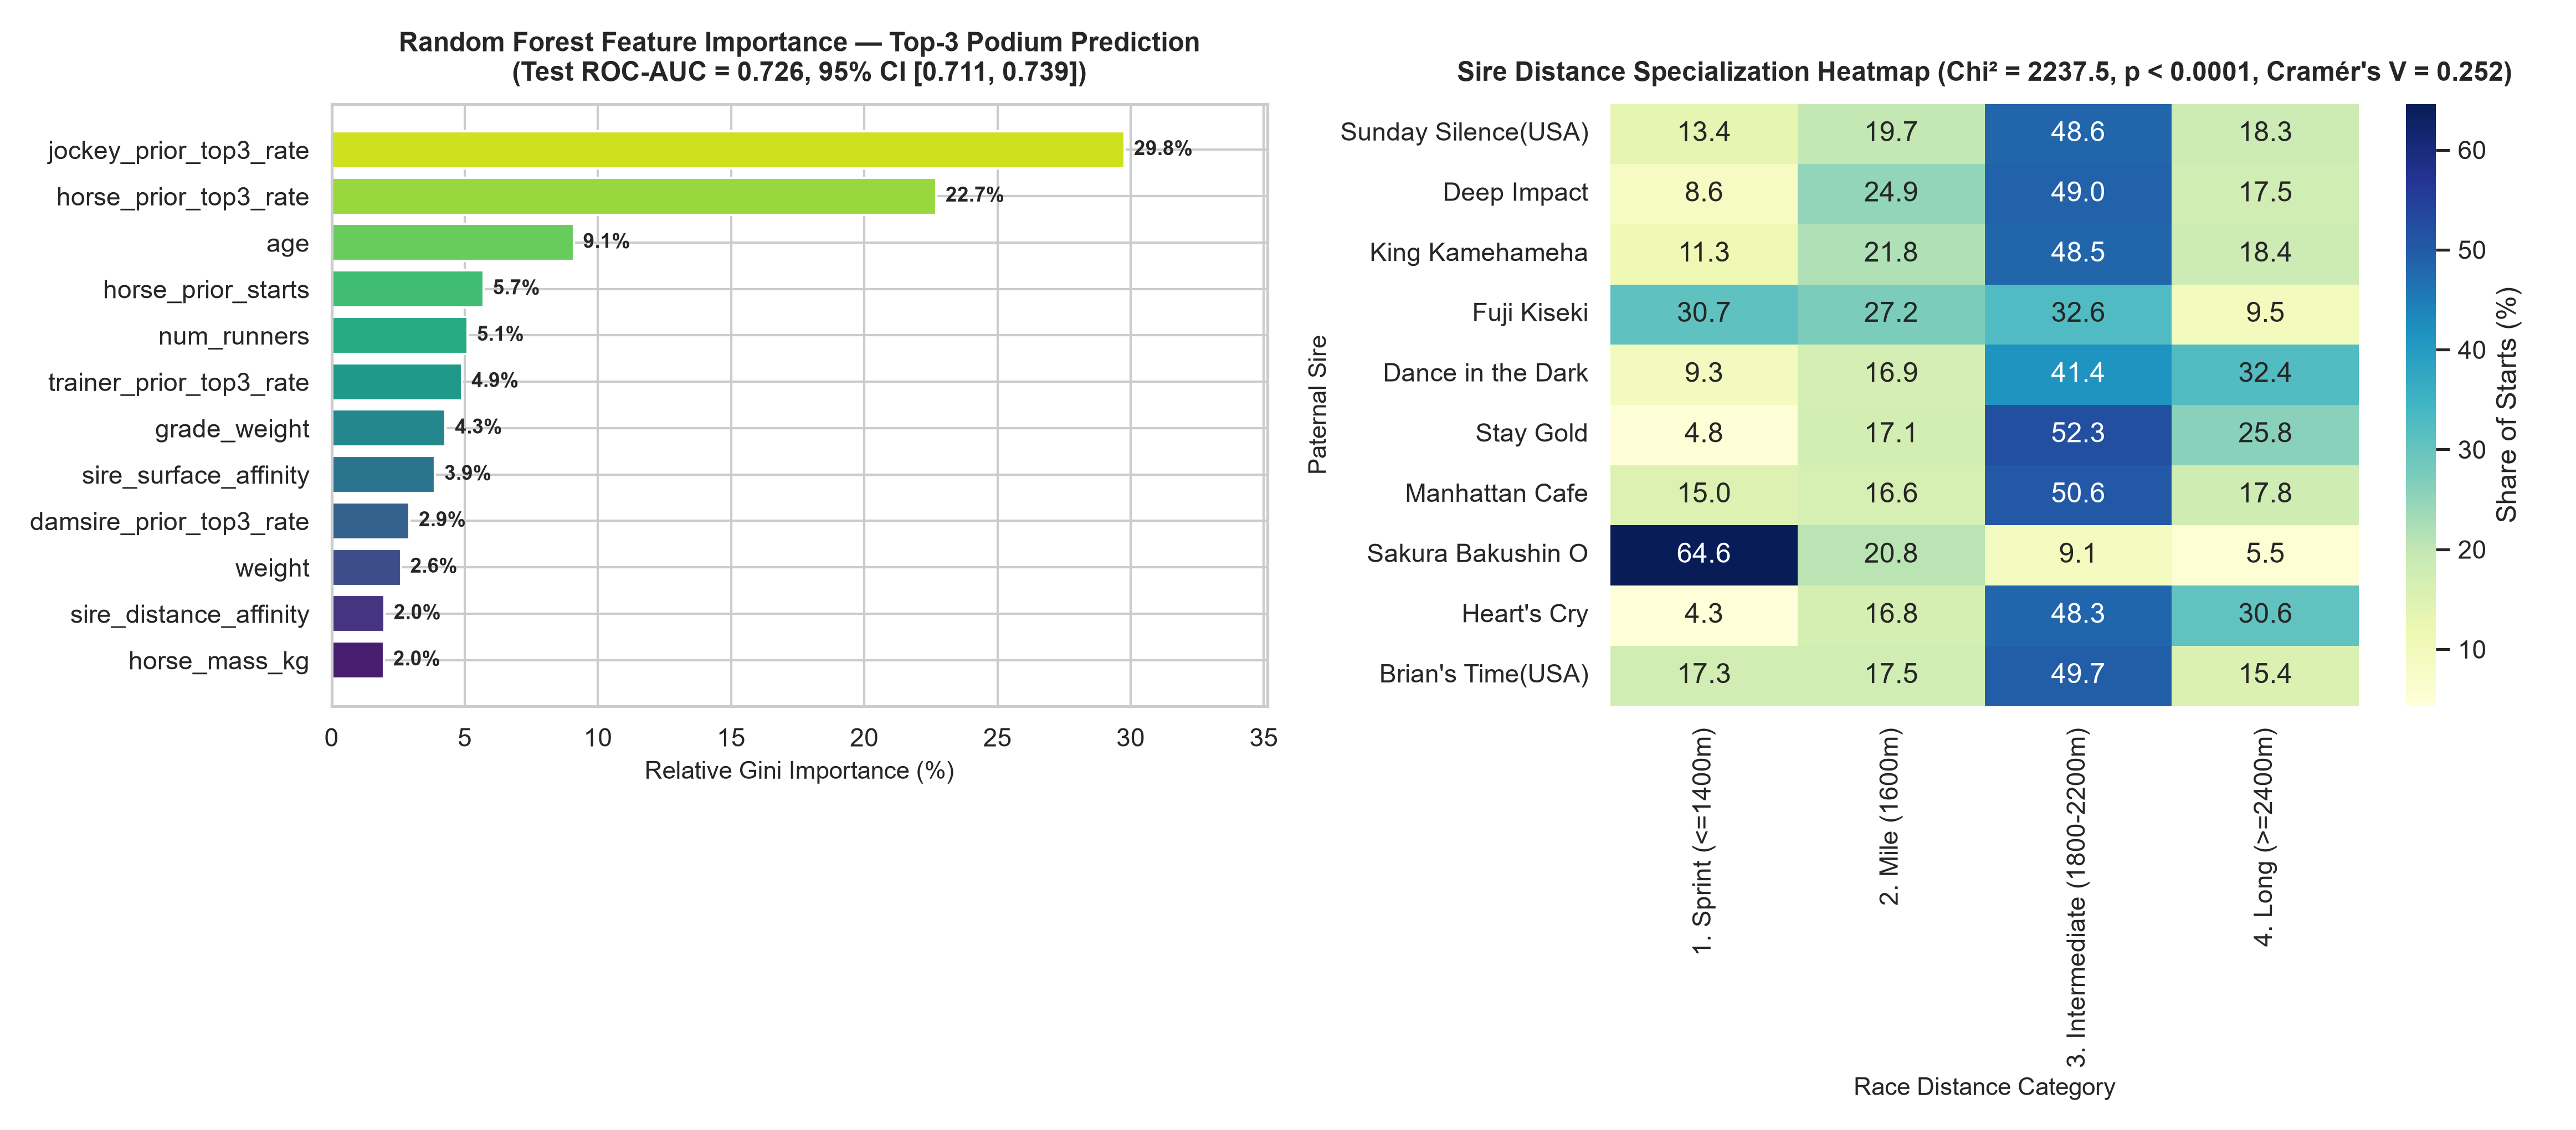
\includegraphics[width=0.94\textwidth]{../assets/ml_random_forest_and_chi2.png}}
\caption{Esquerda: Importância Relativa de Gini (\%)
das variáveis na Random Forest ($\text{ROC-AUC} = 0,7260$). Direita: Mapa de Calor de Especialização por Distância ($\chi^2 = 2237,5, p < 0,0001$).}
\label{fig:rf_chi2}
\end{figure*}

\subsection{Visualização Vetorial em Grafos (Gephi), Suíte Apache Superset e Gamificação TCG}
A modelagem topológica no software \textbf{Gephi} (algoritmo \textit{ForceAtlas2}, Fig.~8) permitiu renderizar em PDF vetorial de zoom infinito quatro estruturas complexas: a Rede de Competição Top 150 PageRank colorida por linhagem paterna, o Fluxo Temporal de Rivalidades Top 500 por Era, o DAG Genealógico de 5 Gerações (4.475 nós de elite mostrando a convergência em funil sobre \textit{Sunday Silence} e \textit{Northern Dancer}) e a Rede Tripartida Jóqueis $\leftrightarrow$ Cavalos $\leftrightarrow$ Treinadores.

\begin{figure}[htbp]
\centerline{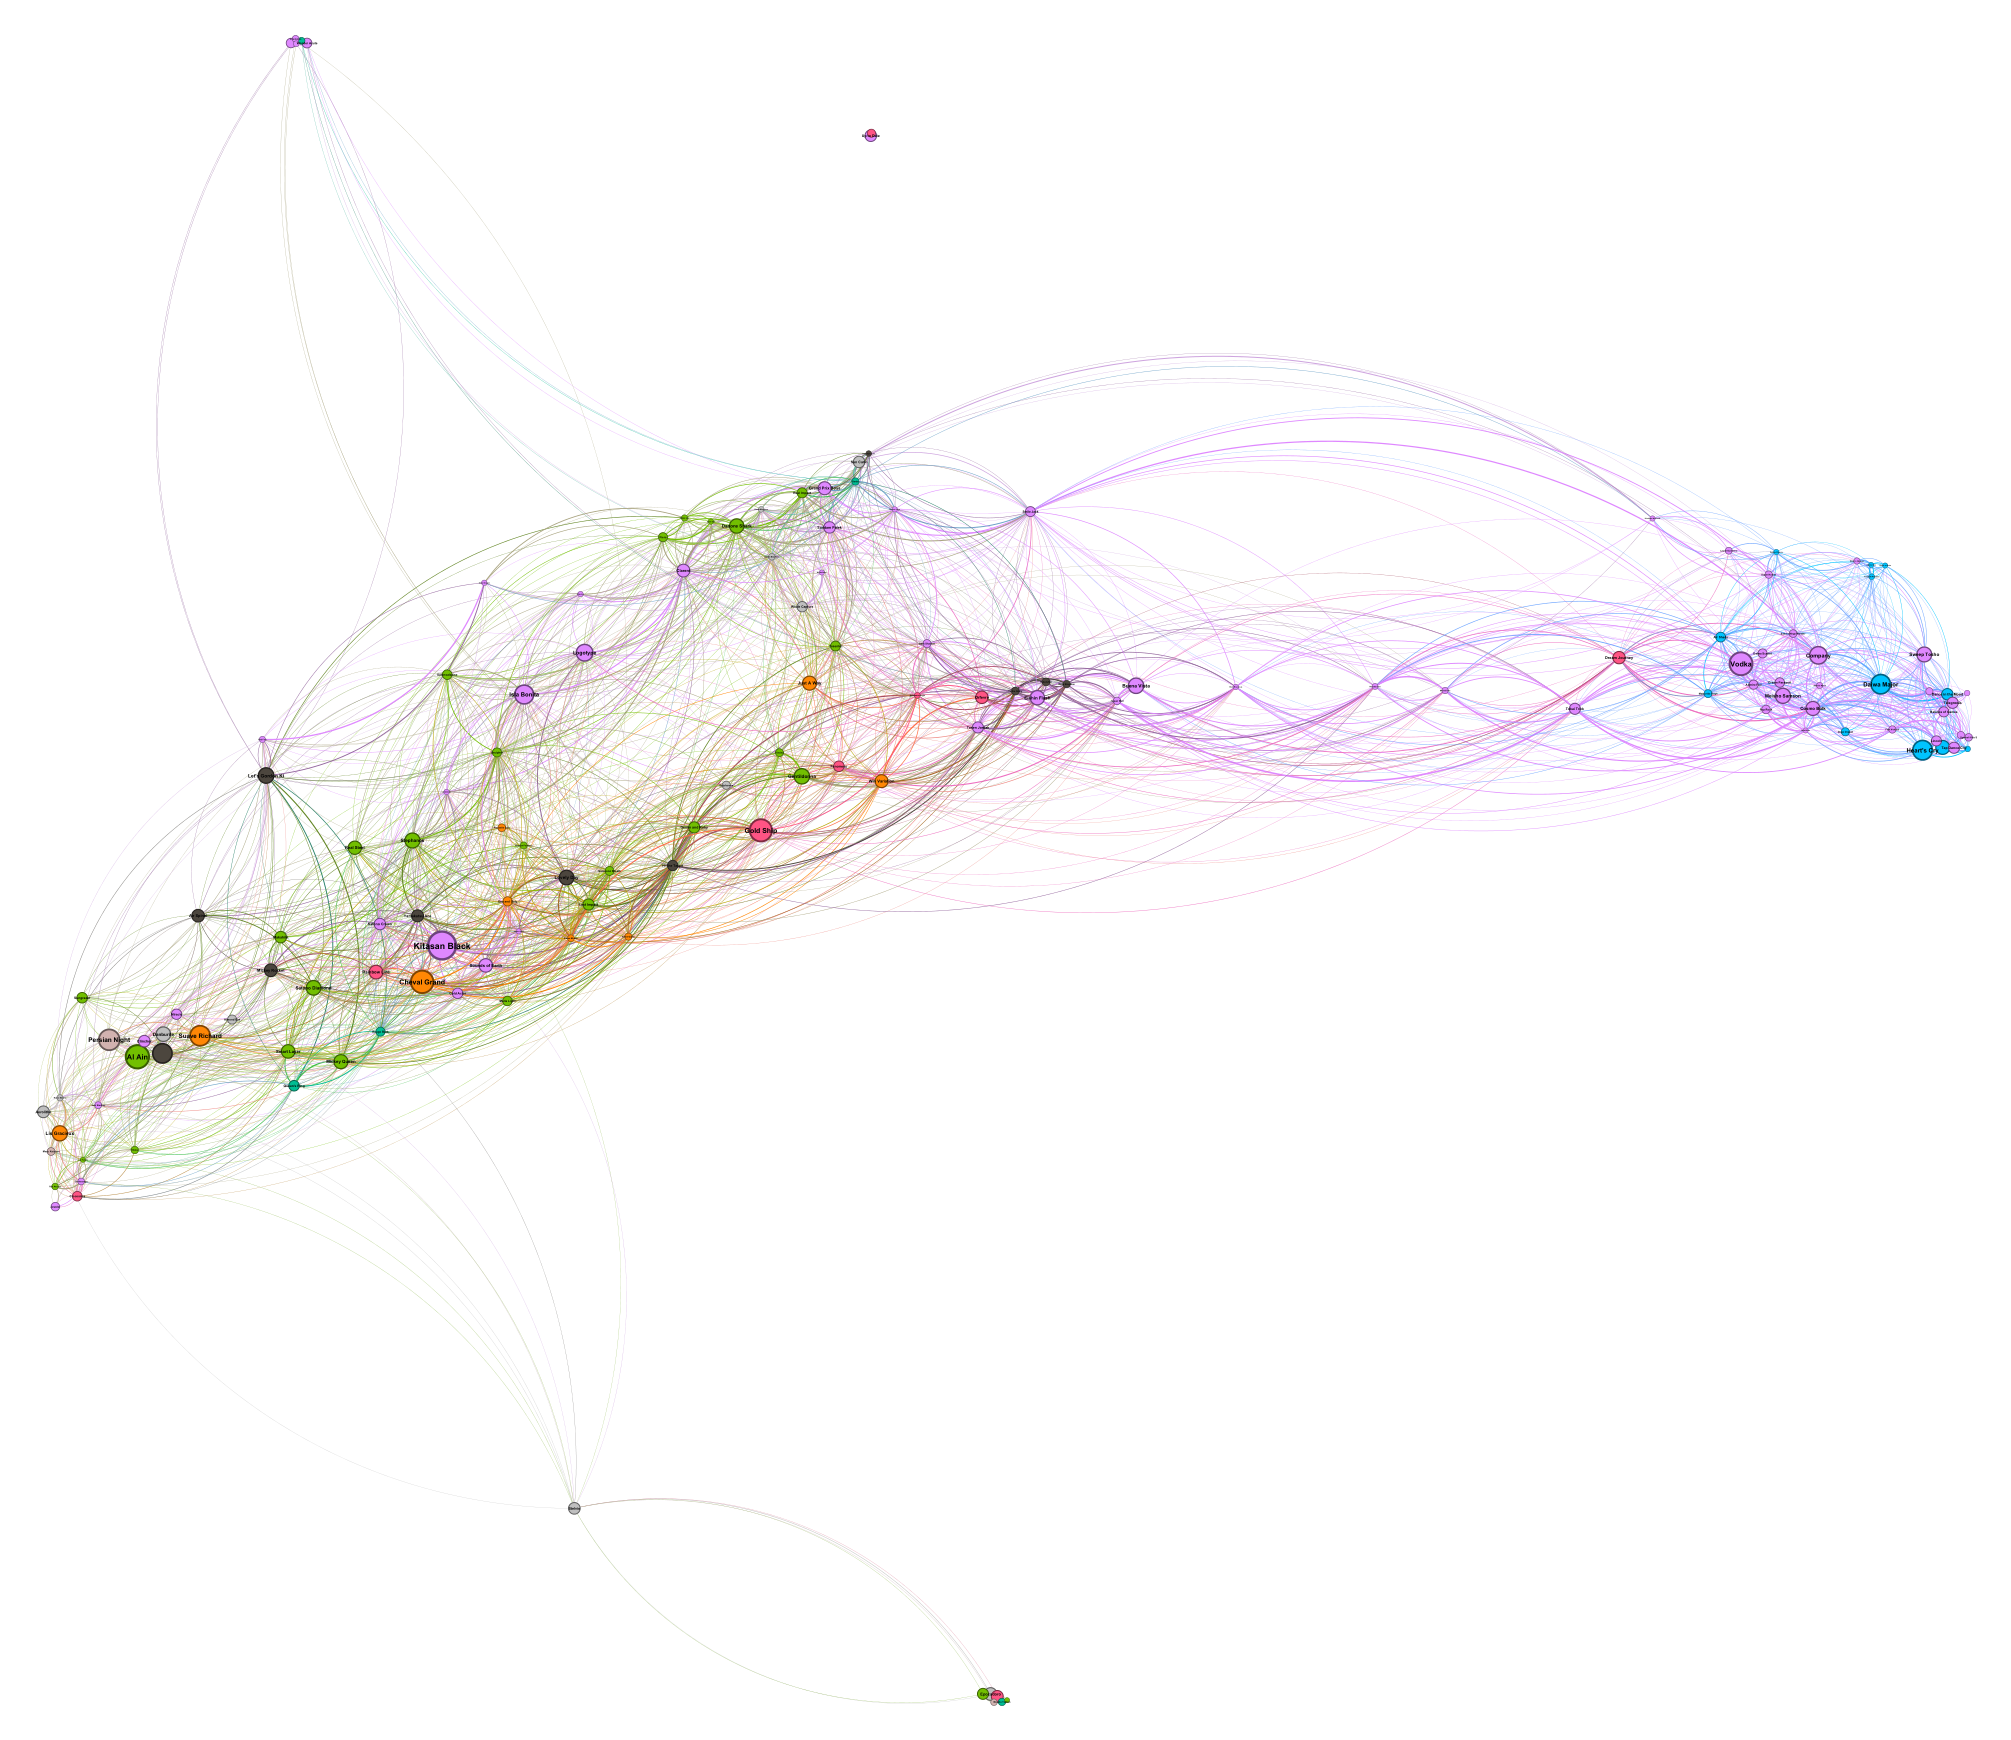
\includegraphics[width=0.49\columnwidth]{../assets/gephi_competition_top150.png}\hfill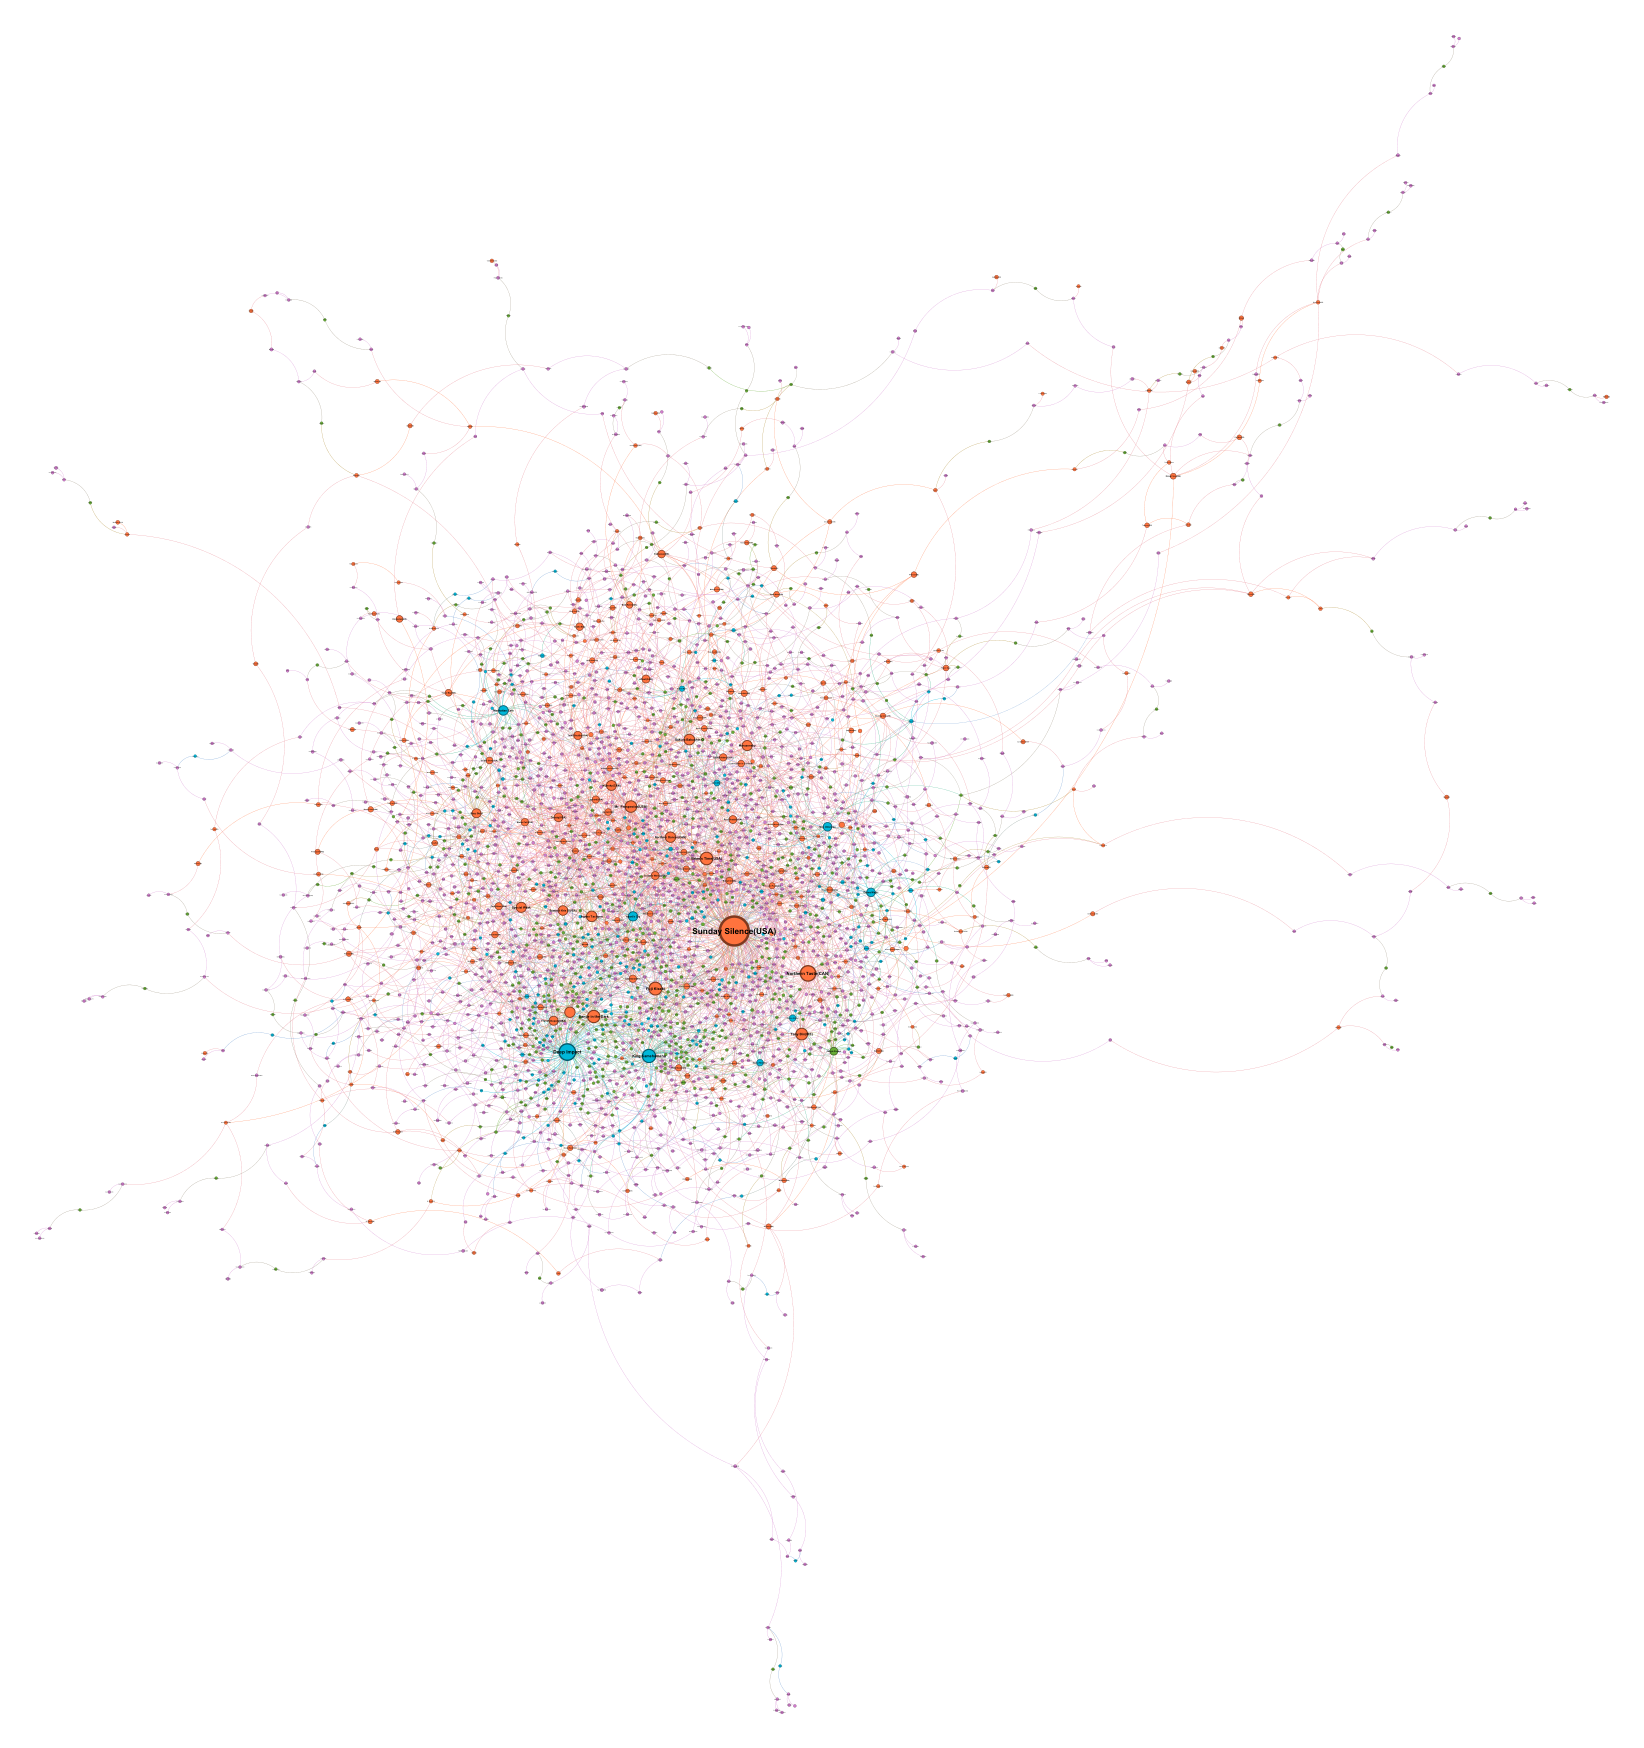
\includegraphics[width=0.49\columnwidth]{../assets/gephi_lineage_dag_elite.png}}
\caption{Redes complexas renderizadas no Gephi (ForceAtlas2). Esquerda: Rede de Competição Top 150 PageRank por linhagem. Direita: Galáxia Genealógica de 5 Gerações (4.475 nós).}
\label{fig:gephi_networks}
\end{figure}

Adicionalmente, implementaram-se duas aplicações web interativas trilíngues (Português, Inglês e Japonês) hospedadas no GitHub Pages:
\begin{enumerate}
    \item \textbf{Suíte Executiva Apache Superset 6.1 / ECharts (\path{docs/superset_interactive_dashboard.html}):} Contém 6 cartões de KPIs e 13 gráficos interativos com suporte a \textit{drill-down} clicável no Sunburst, zoom contínuo no quadrante de PageRank e filtro deslizante ao vivo (\textit{Brush Filter}) nas Coordenadas Paralelas dos 106 garanhões.
    \item \textbf{Arena Gamificada JRA \& JBIS TCG (\path{docs/jra_tcg_arena.html}):} Converteu 520 entidades (324 cavalos, 106 garanhões, 60 jóqueis e 30 patriarcas de 5 gerações) em Cards Colecionáveis com pontuação Overall ($\text{OVR } 76\text{--}99$) e 5 níveis de raridade (\textit{SSR Mythic}, \textit{DIAMOND Anomaly} para os Diamantes Injustiçados com 0 vitórias, \textit{SILVER Crown}, \textit{UR Epic} e \textit{SR Rare}), incluindo modal 3D com árvore genealógica clicável e \textbf{Modo Duelo (VS Mode)} para comparação de polígonos Radar em tempo real.
\end{enumerate}

\section{Repositório de Dados e Reprodutibilidade}
Todo o código-fonte, conjuntos de dados e artefatos visuais estão organizados de forma aberta e reprodutível no repositório GitHub (\url{https://github.com/ImArthz/AEDS2_jra_analysis}) e arquivados permanentemente sob licença \textit{Creative Commons Attribution 4.0} (CC-BY-4.0) no repositório científico europeu \textbf{Zenodo (CERN/OpenAIRE)} sob o identificador digital oficial \textbf{DOI: \texttt{10.5281/zenodo.23681764}} [3]. A arquitetura do repositório compreende:
\begin{itemize}
    \item \path{data/csv/} e \path{data/csv_en/}: As 5 tabelas relacionais exportadas em UTF-8 tanto no japonês original quanto 100\%
traduzidas para o inglês;
    \item \path{data/analysis/}: Tabelas analíticas derivadas (\path{pagerank_full_ranking.csv}, \path{underdog_diamonds_zero_wins.csv}, \path{silver_collectors_zero_g1_wins.csv}, \path{ml_sire_clusters_pca.csv}, \path{ml_feature_importance.csv} e \path{top_inbreeding_ancestors.csv});
    \item \path{data/gephi/}: Os 4 projetos estilizados (\texttt{.gephi}) e os 4 grafos vetoriais de zoom infinito (\texttt{.pdf});
    \item \path{src/}: Os 12 módulos Python do pipeline (\path{scraper_jra.py}, \path{scraper_pedigree.py}, \path{clean_data.py}, \path{hybrid_translator.py}, \path{translate_db.py}, \path{validate_data.py}, \path{graph_analysis.py}, \path{export_gephi.py}, \path{ml_analysis.py}, \path{generate_advanced_viz.py}, \path{generate_tcg_cards.py} e \path{run_pipeline.py});
    \item \path{.github/workflows/compile_latex.yml}: Pipeline de Integração e Entrega Contínua (CI/CD) via \textit{GitHub Actions} que regenera os dashboards interativos e compila automaticamente os documentos LaTeX via \texttt{XeLaTeX} a cada \textit{push}, publicando os PDFs e HTMLs na aba \textit{Releases}.
\end{itemize}

\section{Conclusão e Considerações Finais}
Este trabalho demonstrou como a integração rigorosa entre Engenharia de Dados, Inteligência Artificial Generativa (para tradução semântica de domínio complexo), Teoria dos Grafos, Estatística Inferencial, Aprendizado de Máquina e Visualização Multidimensional permite extrair conhecimento científico inédito de bases históricas legadas e ruidosas.

Respondendo à questão central da pesquisa, comprovou-se empiricamente que: (i) a herança genética de 5 gerações determina com significância estatística extrema ($\chi^2 = 2237,5, p < 10^{-300}$) o nicho físico de superfície e distância em que o Puro-Sangue é competitivo, estruturando os reprodutores em 4 arquétipos bem definidos (63,4\%
de variância em 2 eixos PCA) e revelando dimorfismo biométrico entre competidores de areia ($\approx 496\text{ kg}$) e grama ($\approx 477\text{ kg}$); (ii) o fator humano (retrospecto prévio do jóquei com 29,8\%
de importância de Gini e do treinador com 4,9\%)
aliado à forma atlética prévia do animal (22,7\%)
governa a predição de pódio em corridas futuras ($\text{ROC-AUC} = 0,7260$ sem vazamento temporal); e (iii) a centralidade PageRank em grafos corrige a miopia da contagem simples de vitórias ao resgatar ``Diamantes Injustiçados'' como \textit{Sounds of Earth} (\#32 geral entre 8.135 cavalos com zero vitórias Graded). Por fim, a tradução dessa matriz matemática para o dashboard interativo em \textit{Apache Superset / ECharts} e para a arena gamificada de 520 cards colecionáveis comprova o potencial da visualização de dados para tornar modelos complexos acessíveis, intuitivos e interativos para qualquer público.

\begin{thebibliography}{10}
\bibitem{jra_official} Japan Racing Association (JRA), ``JRA Official Historical Graded Races Database (\textit{Jusho} 2002--2025),'' Tokyo, Japan. [Online]. Available: \url{https://www.jra.go.jp/}
\bibitem{jbis_official} Japan Bloodhorse Breeders' Association (JBBA), ``Japan Bloodhorse Information System (JBIS) 5-Generation Pedigree Records,'' Tokyo, Japan. [Online]. Available: \url{https://www.jbis.or.jp/}
\bibitem{mendonca_zenodo} A. D. O. Mendonça, ``JRA Graded Races (2002--2025) \& JBIS 5-Generation Pedigree Dataset (Bilingual JA/EN + Graph Networks \& ML),'' \textit{Zenodo}, v2.0.0, 2026, doi: 10.5281/zenodo.23681764.
\bibitem{wright1922} S. Wright, ``Coefficients of Inbreeding and Relationship,'' \textit{The American Naturalist}, vol. 56, no. 645, pp. 330--338, 1922.
\bibitem{pagerank1999} L. Page, S. Brin, R. Motwani, and T. Winograd, ``The PageRank Citation Ranking: Bringing Order to the Web,'' Stanford InfoLab, Tech. Rep. 1999-66, 1999.
\bibitem{breiman2001} L. Breiman, ``Random Forests,'' \textit{Machine Learning}, vol. 45, no. 1, pp. 5--32, 2001.
\bibitem{arthur2007} D. Arthur and S. Vassilvitskii, ``k-means++: The Advantages of Careful Seeding,'' in \textit{Proc. ACM-SIAM Symp. Discrete Algorithms (SODA)}, 2007, pp. 1027--1035.
\bibitem{datavizproject} Ferdio, ``DataViz Project --- Collection of Data Visualizations to Get Inspired and Finding the Right Type,'' 2026. [Online]. Available: \url{https://datavizproject.com/}
\bibitem{superset} Apache Software Foundation, ``Apache Superset 6.1 \& Apache ECharts 5.5 Modern Data Exploration and Visualization Platform,'' 2026. [Online]. Available: \url{https://superset.apache.org/}
\bibitem{gephi2009} M. Bastian, S. Heymann, and M. Jacomy, ``Gephi: An Open Source Software for Exploring and Manipulating Networks,'' in \textit{Proc. Int. AAAI Conf. Weblogs and Social Media (ICWSM)}, 2009, pp. 361--362.
\end{thebibliography}

\end{document}
